
\newpage
\subsection{Observations of the size of hidden layers}

An interesting phenomenon is that if we increase the size of the hidden layer, the two-layer linear NN descend faster from the beginning than single-layer linear NN. We use 0 and 1 in MNIST dataset to observe if this phenomenon also occurs in MNIST dataset.

\begin{figure}[H]
	\centering
	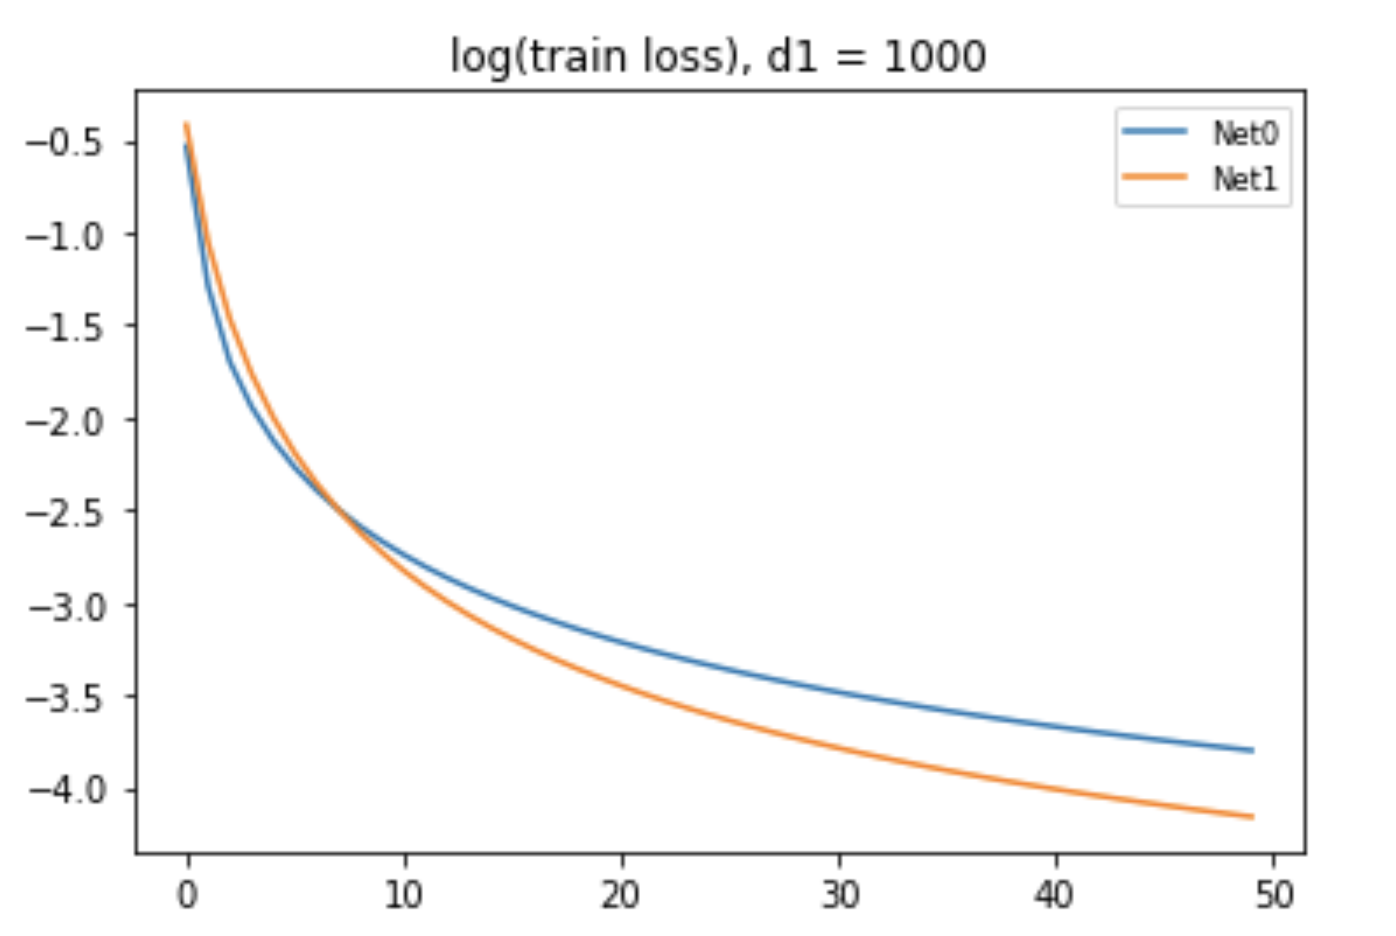
\includegraphics[width=2.5in]{MNIST_hidden1000_step50.png}
	\caption{MNIST: $d_1 = 1000, lr = 0.1$}
\end{figure}


\begin{figure}[H]
	\centering
	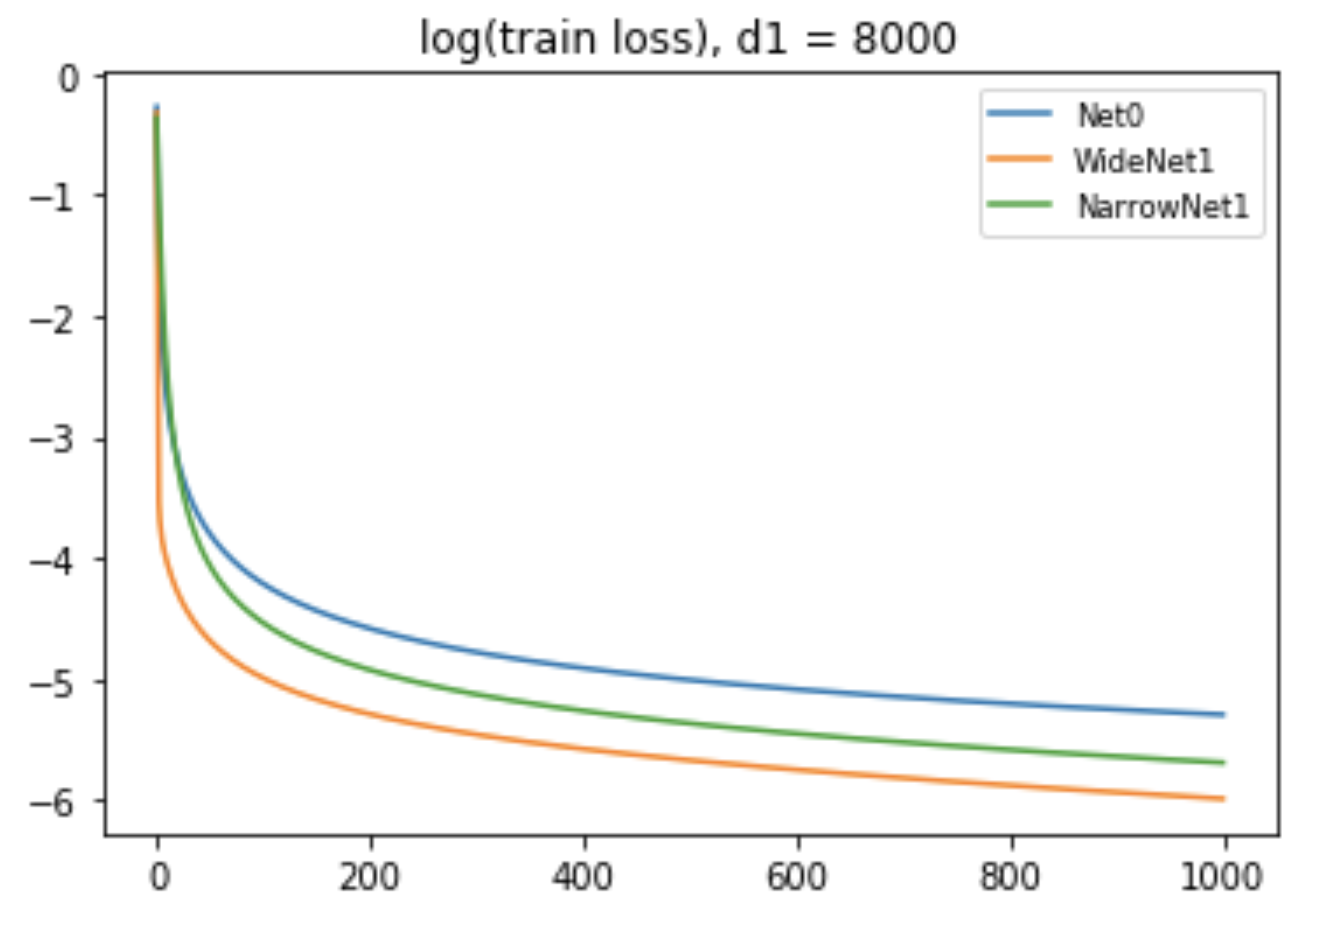
\includegraphics[width=2in]{MNIST_hidden8000_step1000.png}
	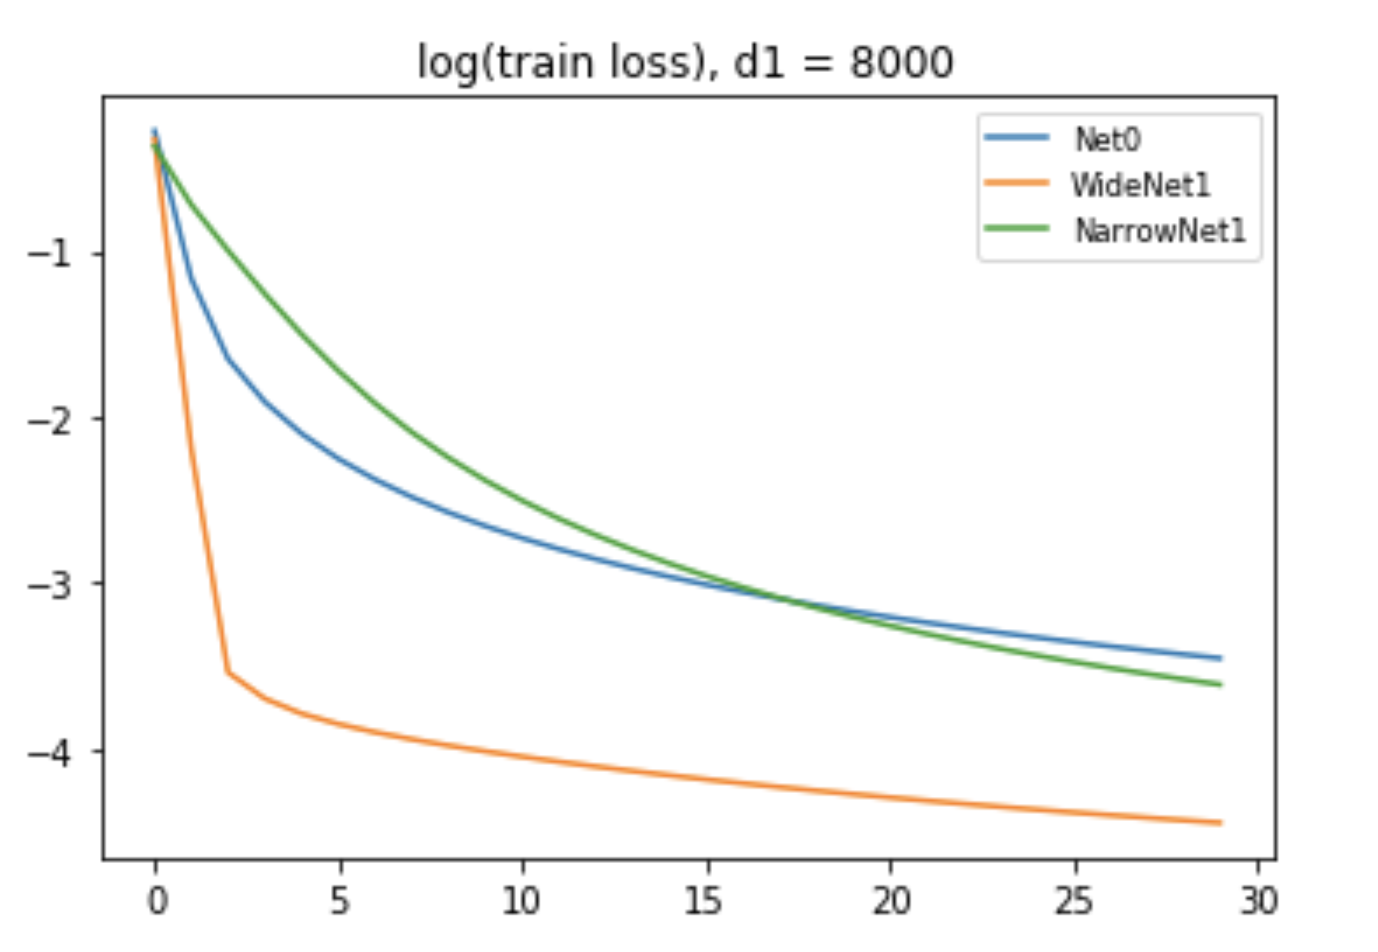
\includegraphics[width=2in]{MNIST_hidden8000_step30.png}
	\caption{MNIST: WideNet($d_1 = 8000$) vs NarrowNet($d_1 = 100$)}
\end{figure}

\begin{figure}[H]
	\centering
	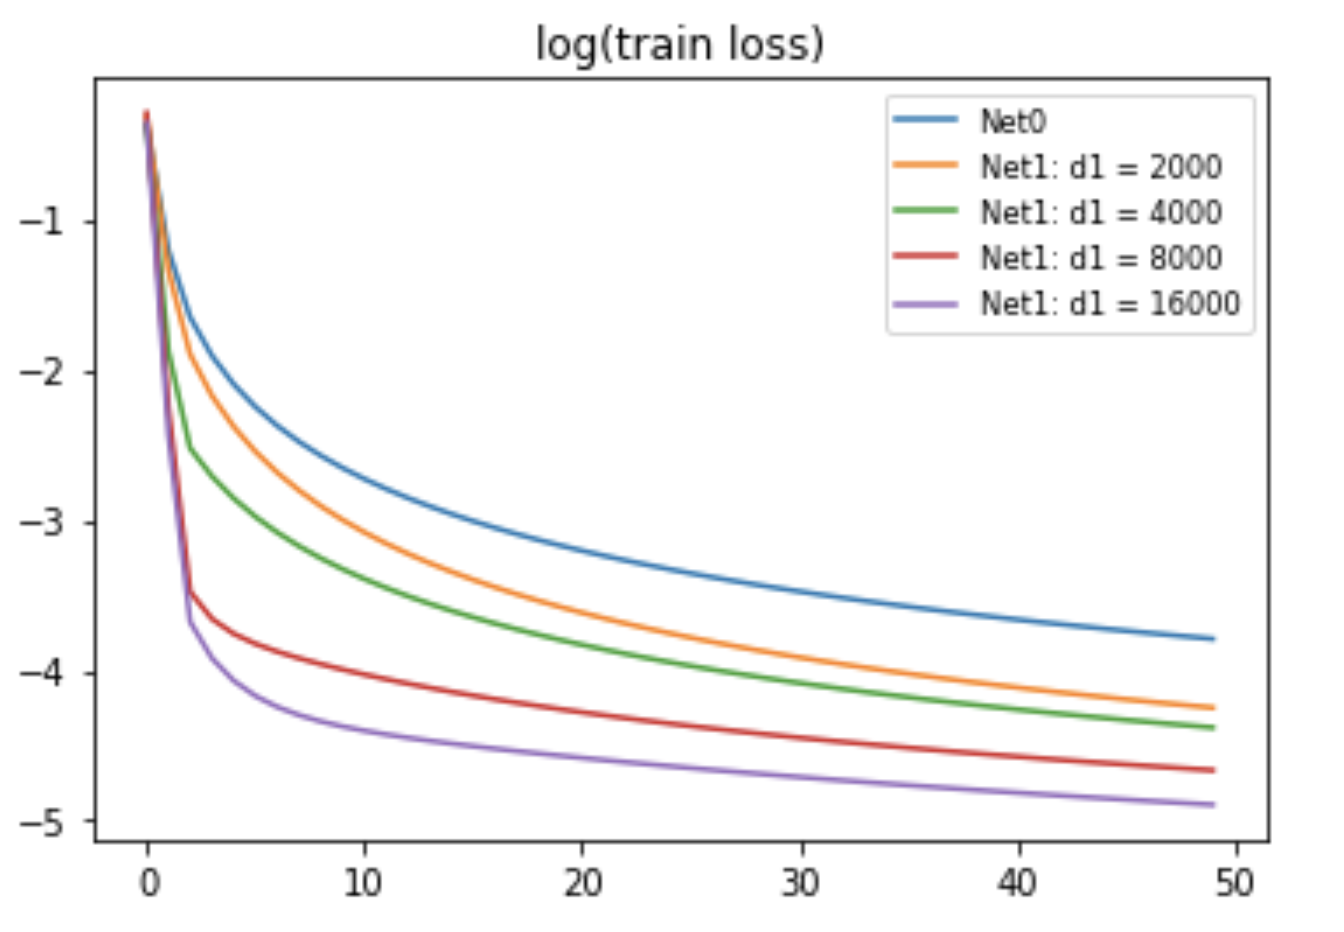
\includegraphics[width=2in]{MNIST_hidden64000_1.png}
	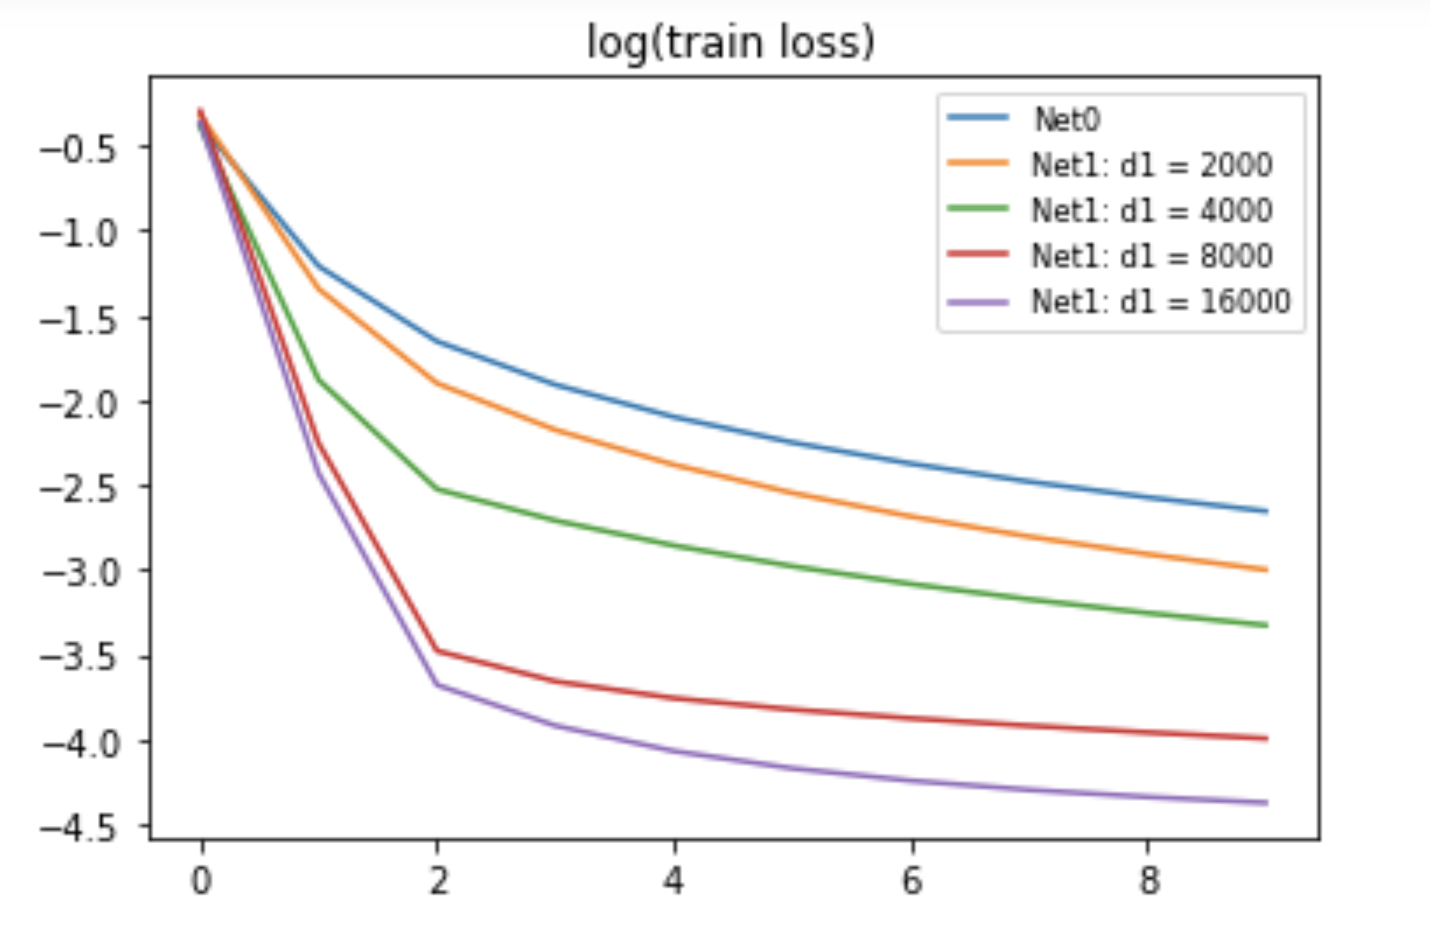
\includegraphics[width=2in]{MNIST_hidden64000_2.png}
	\caption{MNIST: $d_1 = 2000,4000,8000,16000$}
\end{figure}

\begin{figure}[H]
	\centering
	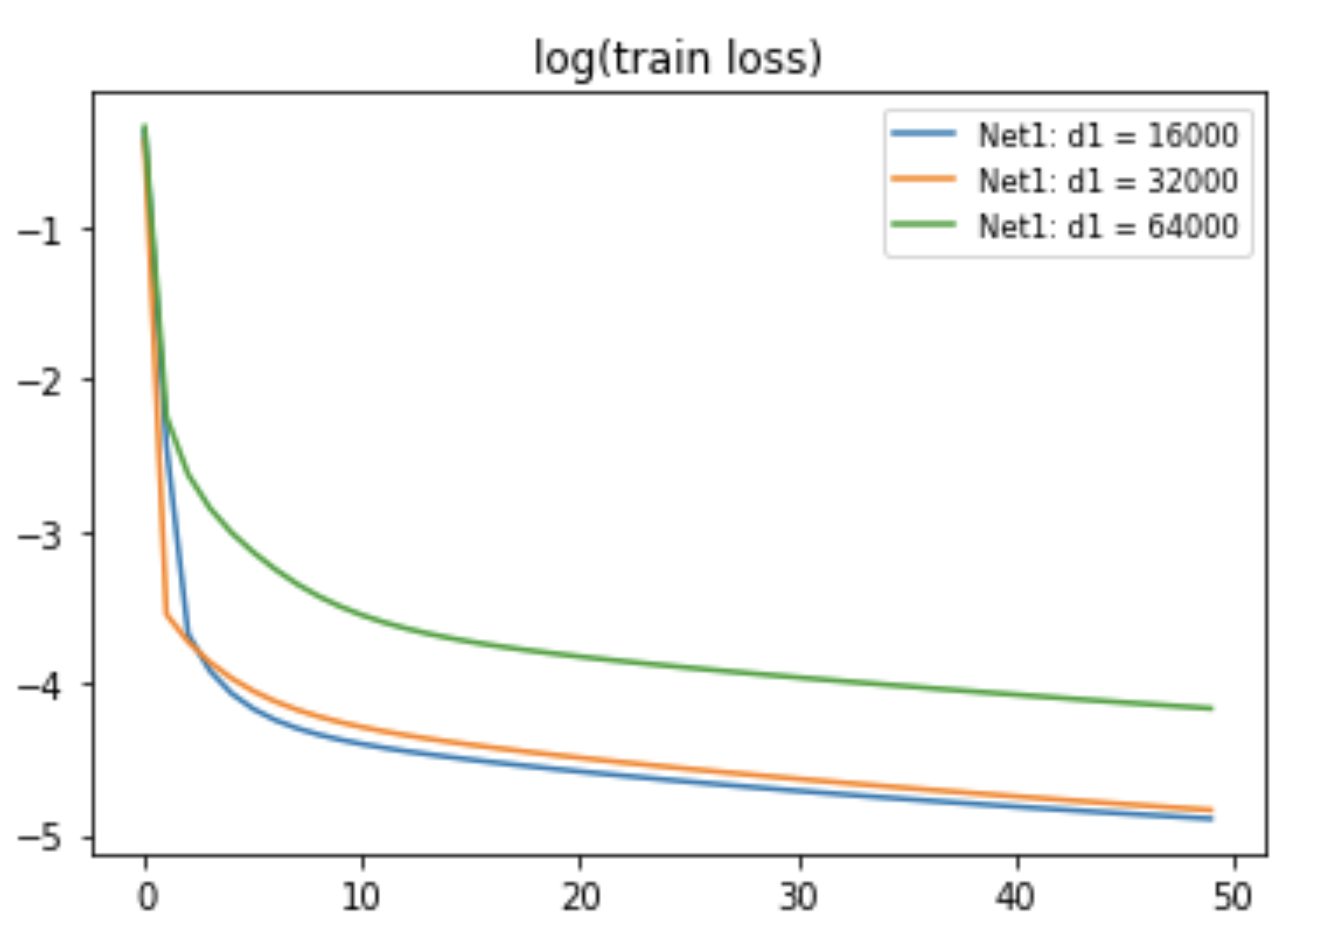
\includegraphics[width=2in]{MNIST_hidden64000_3.png}
	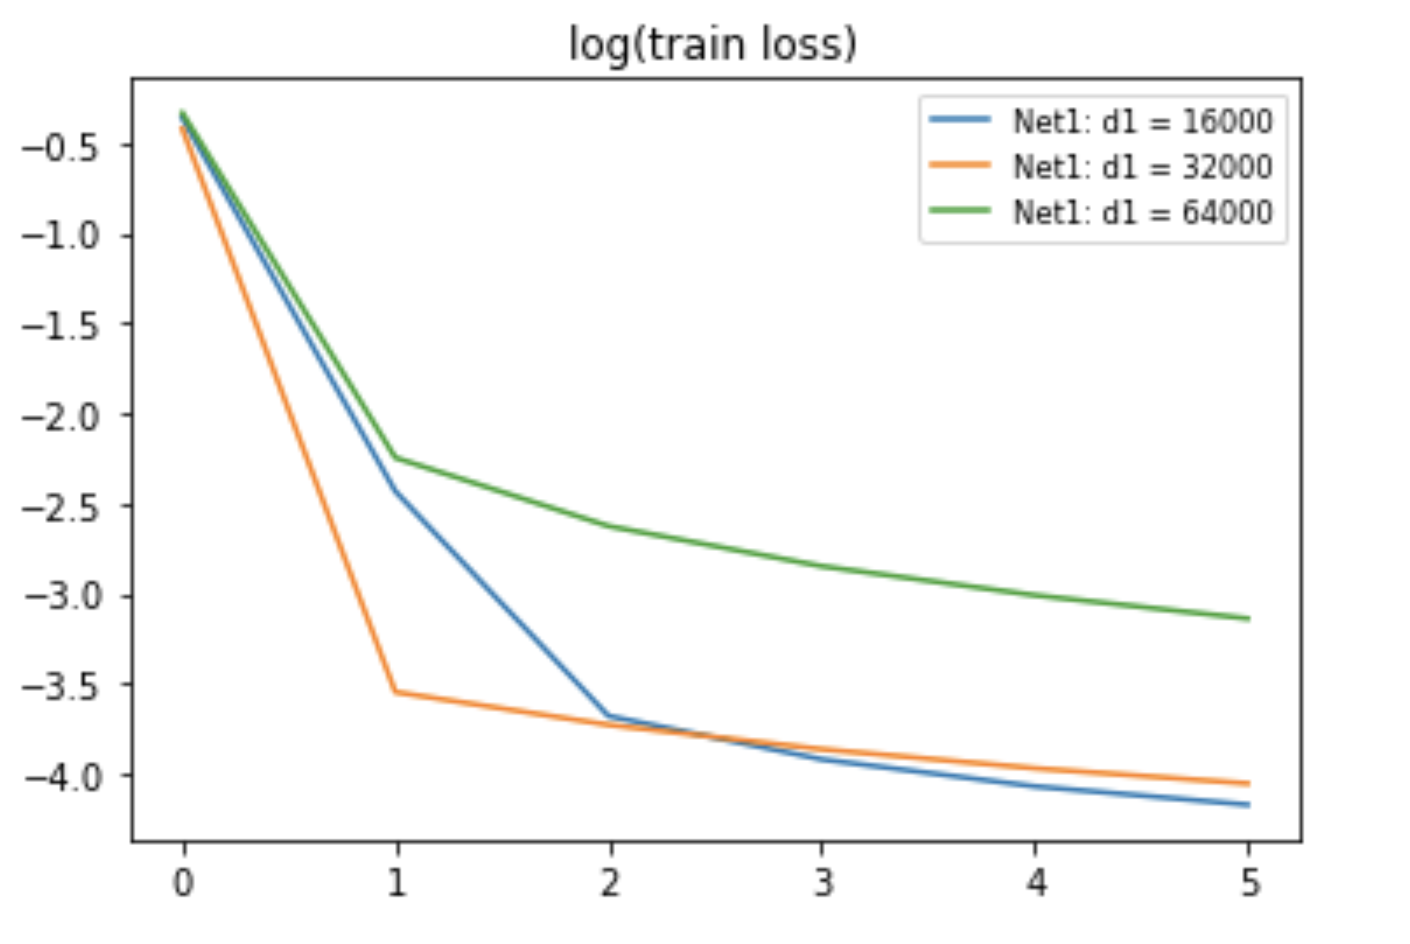
\includegraphics[width=2in]{MNIST_hidden64000_4.png}
	\caption{MNIST: $d_1 = 16000, 32000, 64000$}
\end{figure}

\begin{itemize}
	\item When $d_1 = 1000$, Net1 descend slower than single-layer linear NN from the beginning, but catch up and surpass Net0
	\item When $d_1 > 2000$, Net1 descend faster than Net0 from the beginning. And the speed goes faster as we increase the size of hidden-layer $d_1$.
	\item If we put Net0(Single-layer), NarrowNet1(2-layer with $d_1 = 100$), WideNet1(2-layer with $d_1 = 8000$) together, we can observe that Net0 descend faster at the beginning than NarrowNet1, but NarrowNet1 catches up and surpass Net0 soon. WideNet1 is much more faster than the other two at the beginning and remain the fastest all the time.
\end{itemize}

\subsection{Observation of initializations}

But if we look at how Pytorch do initialization, we can see that their initialization method is related to the size of hidden layer. For example, for some layer in linear NN, if input size is $d_{in}$, output size is $d_{out}$, then Pytorch use the following initialization:
\begin{equation}
	W,b \sim U(-\frac{1}{\sqrt{d_{in}}},\frac{1}{\sqrt{d_{in}}}),
\end{equation}
 which means each single parameter in $W$ and $b$ is uniformly sampled from interval $(-\frac{1}{\sqrt{d_{in}}},\frac{1}{\sqrt{d_{in}}})$.\\
 
 We know that in our experiments, there are mainly three things that determine the training process: (1) the size of hidden layer, (2) Initialization, (3) learning rate(step size). But if we use a default initialization, we are hard to draw a conclusion because we don't know if this kind of initializaiton is the best in different hidden-size settings. So we do a simple experiment to test this. \\
 \indent We only consider a 2-layer linear NN where the fisrt layer is unbiased. So we need to initialize the parameters $W_1,W_2,b$. We set
 \begin{equation}
 	W_1,W_2,b \sim U(-\beta,\beta),
 \end{equation}
 and change the value of $\beta$, to see if it will influence the descent of loss.
 
  \begin{figure}[H]
 	\centering
 	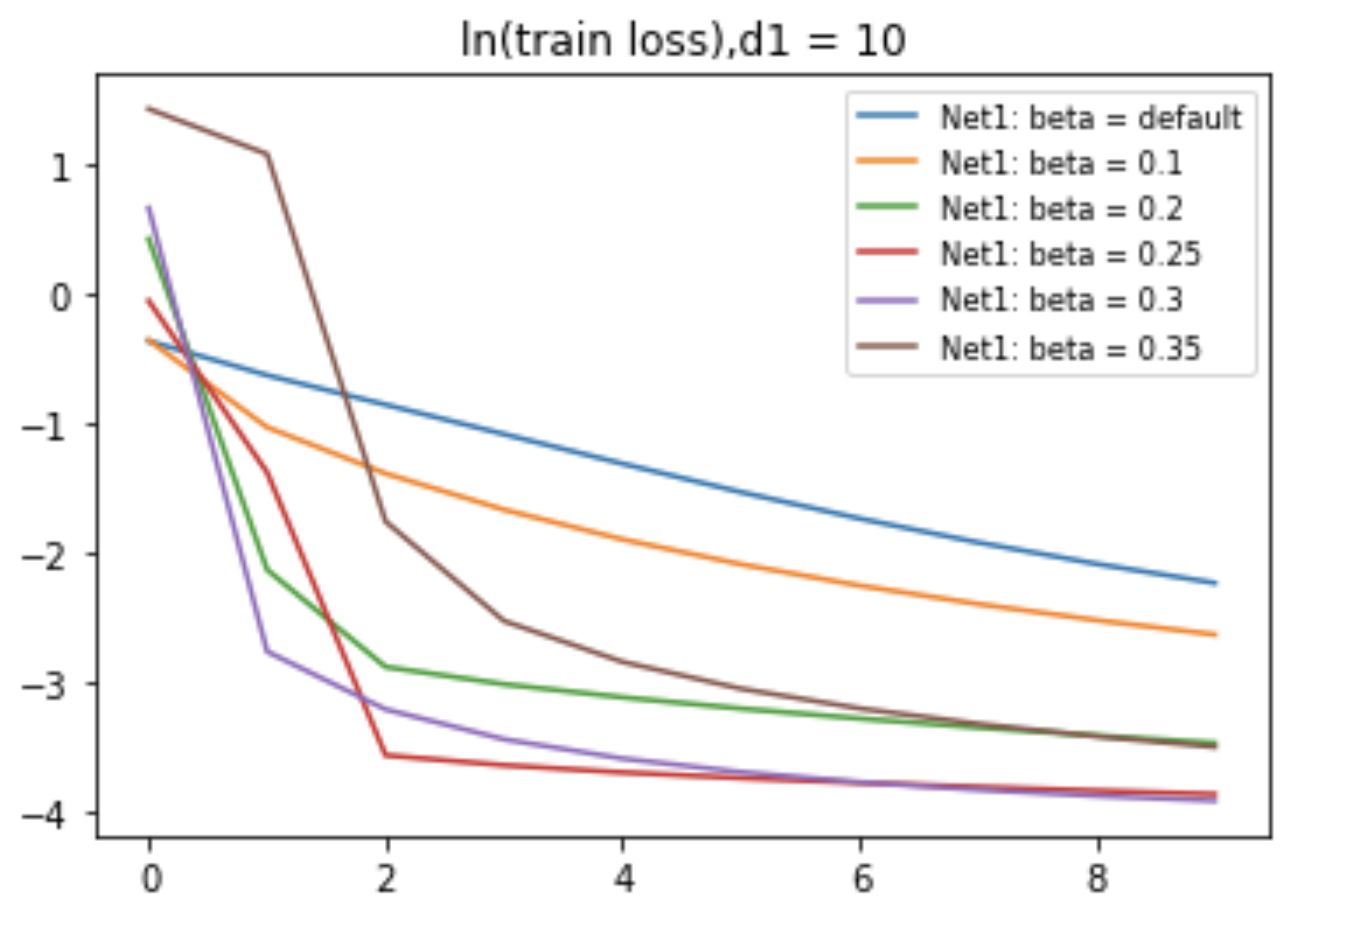
\includegraphics[width=1.5in]{MNIST_hidden10_uniform1.png}
 	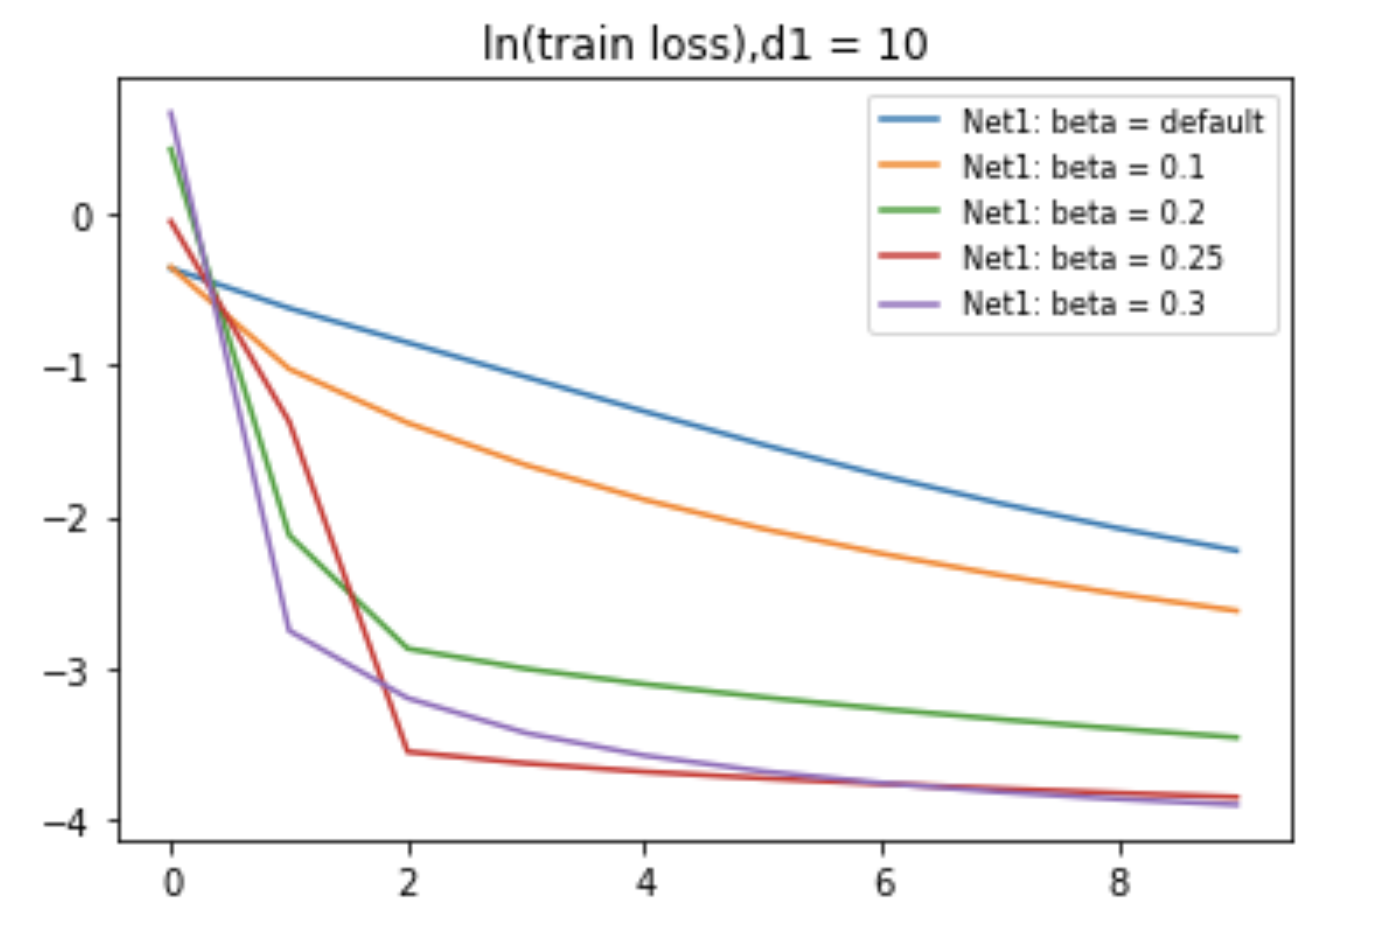
\includegraphics[width=1.5in]{MNIST_hidden10_uniform2.png}
 	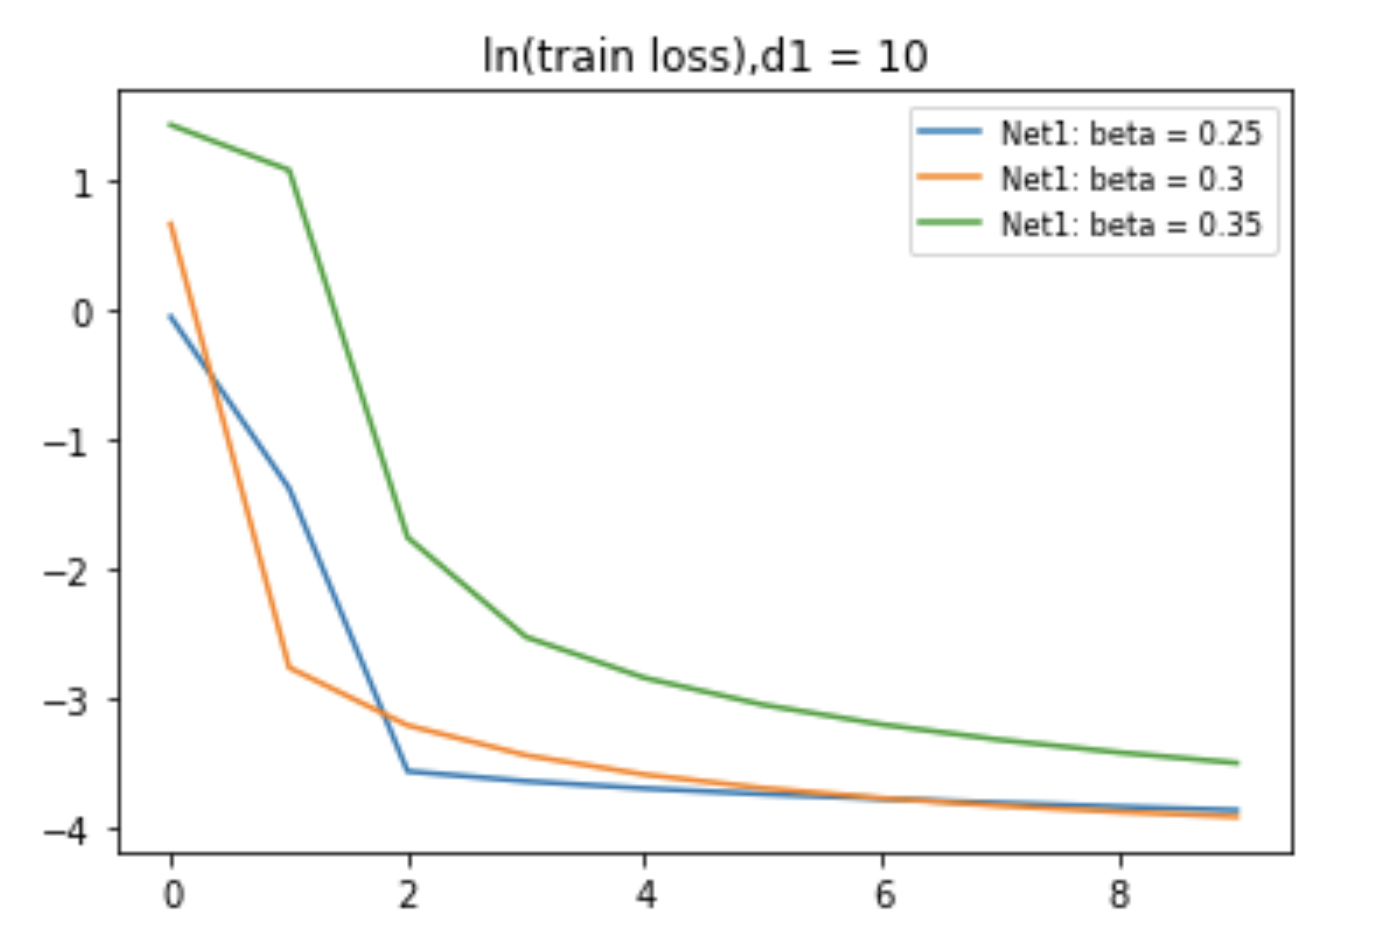
\includegraphics[width=1.5in]{MNIST_hidden10_uniform3.png}
 	\caption{MNIST: $d_1 = 10$, $W_1,W_2,b \sim U(-\beta,\beta)$}
 \end{figure}

 \begin{figure}[H]
 	\centering
 	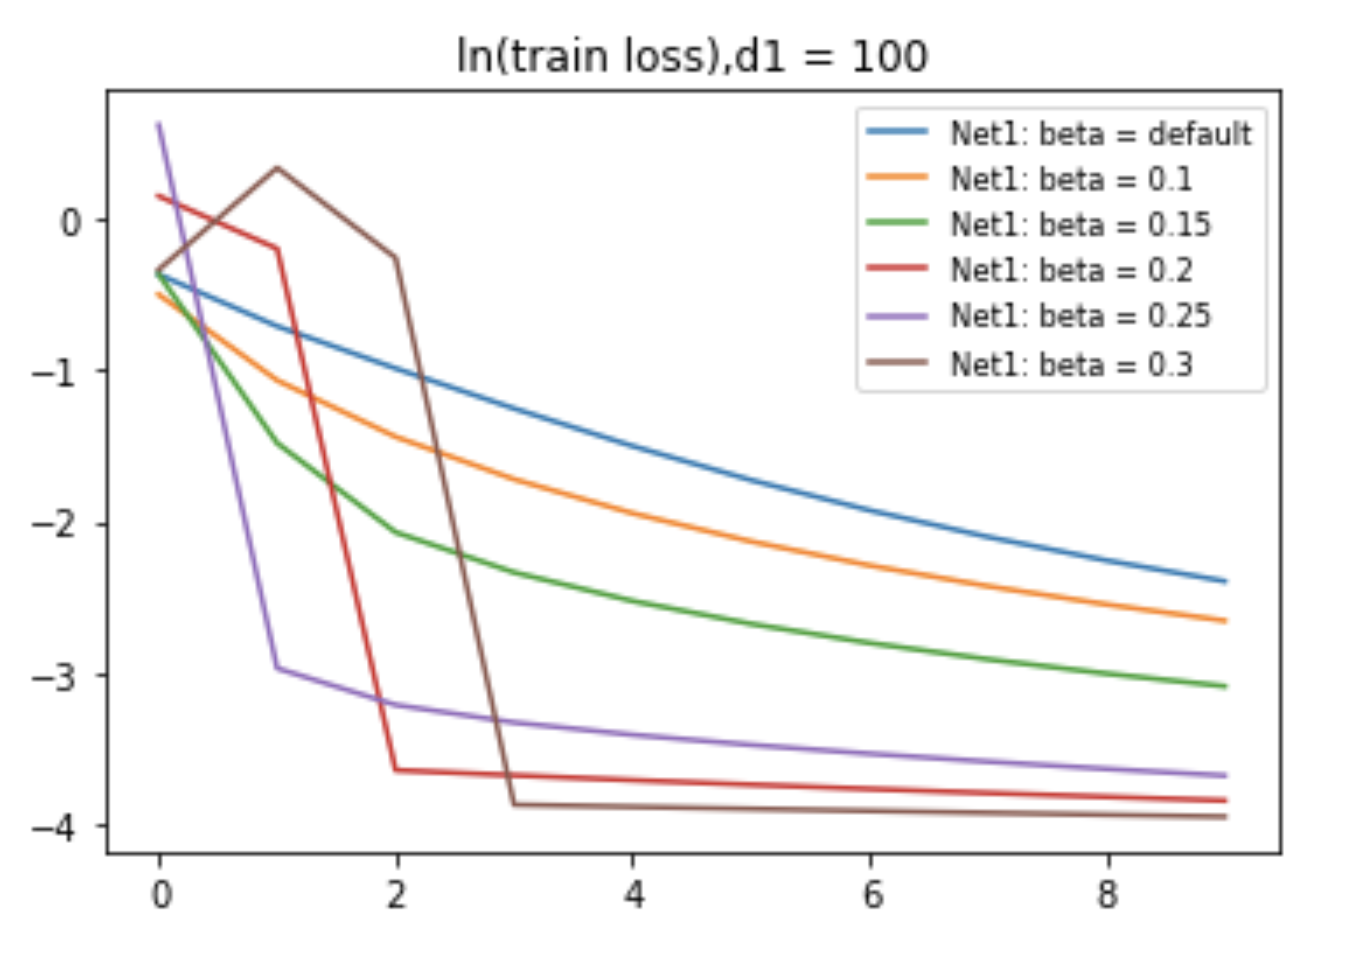
\includegraphics[width=1.5in]{MNIST_hidden100_uniform1.png}
 	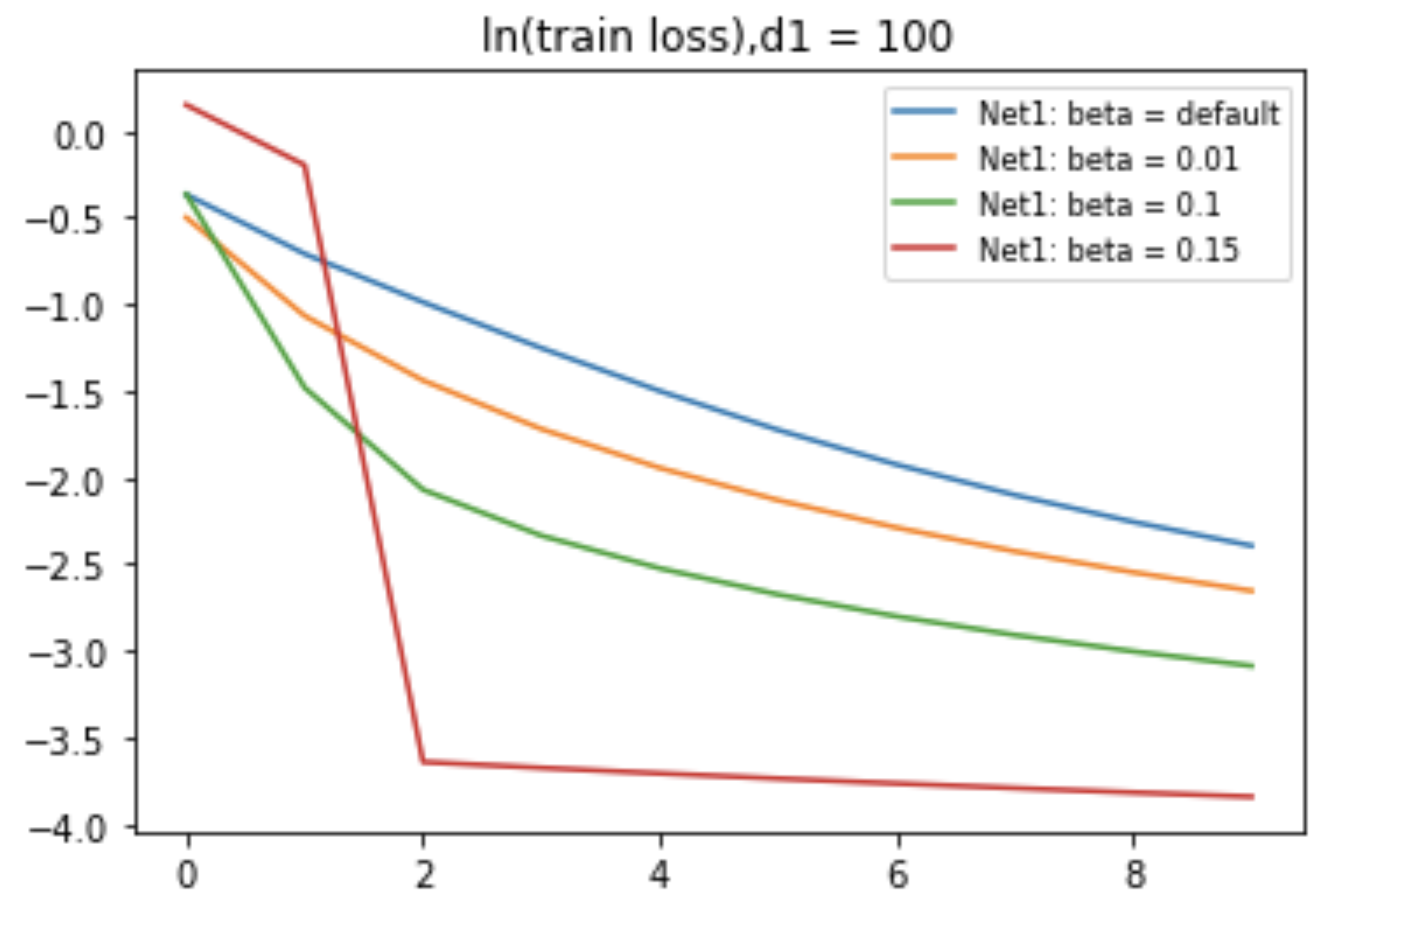
\includegraphics[width=1.5in]{MNIST_hidden100_uniform2.png}
 	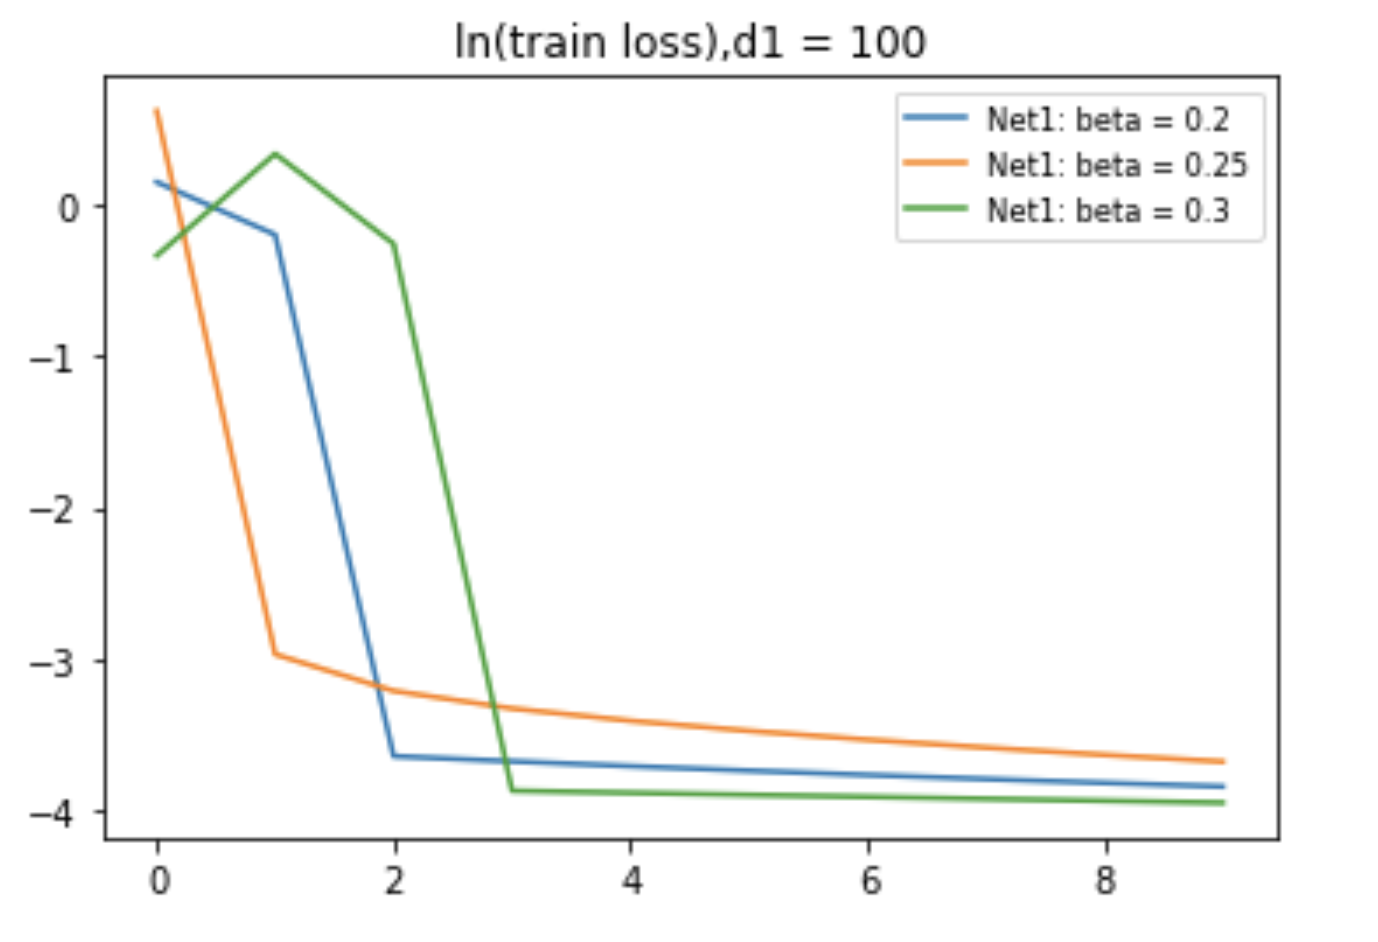
\includegraphics[width=1.5in]{MNIST_hidden100_uniform3.png}
 	\caption{MNIST: $d_1 = 100$, $W_1,W_2,b \sim U(-\beta,\beta)$}
 \end{figure}

 \begin{figure}[H]
	\centering
	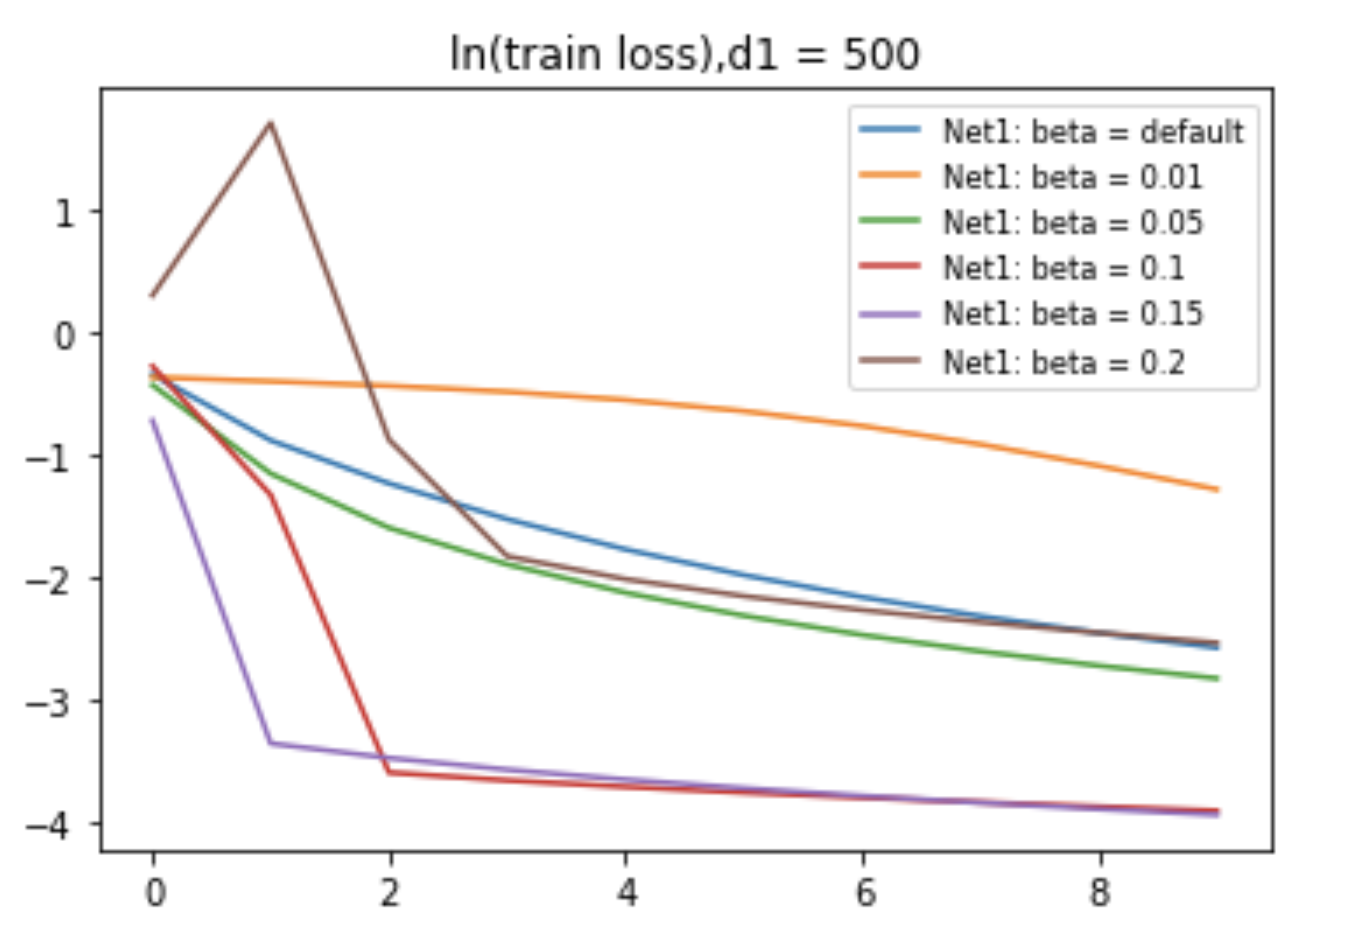
\includegraphics[width=1.5in]{MNIST_hidden500_uniform1.png}
	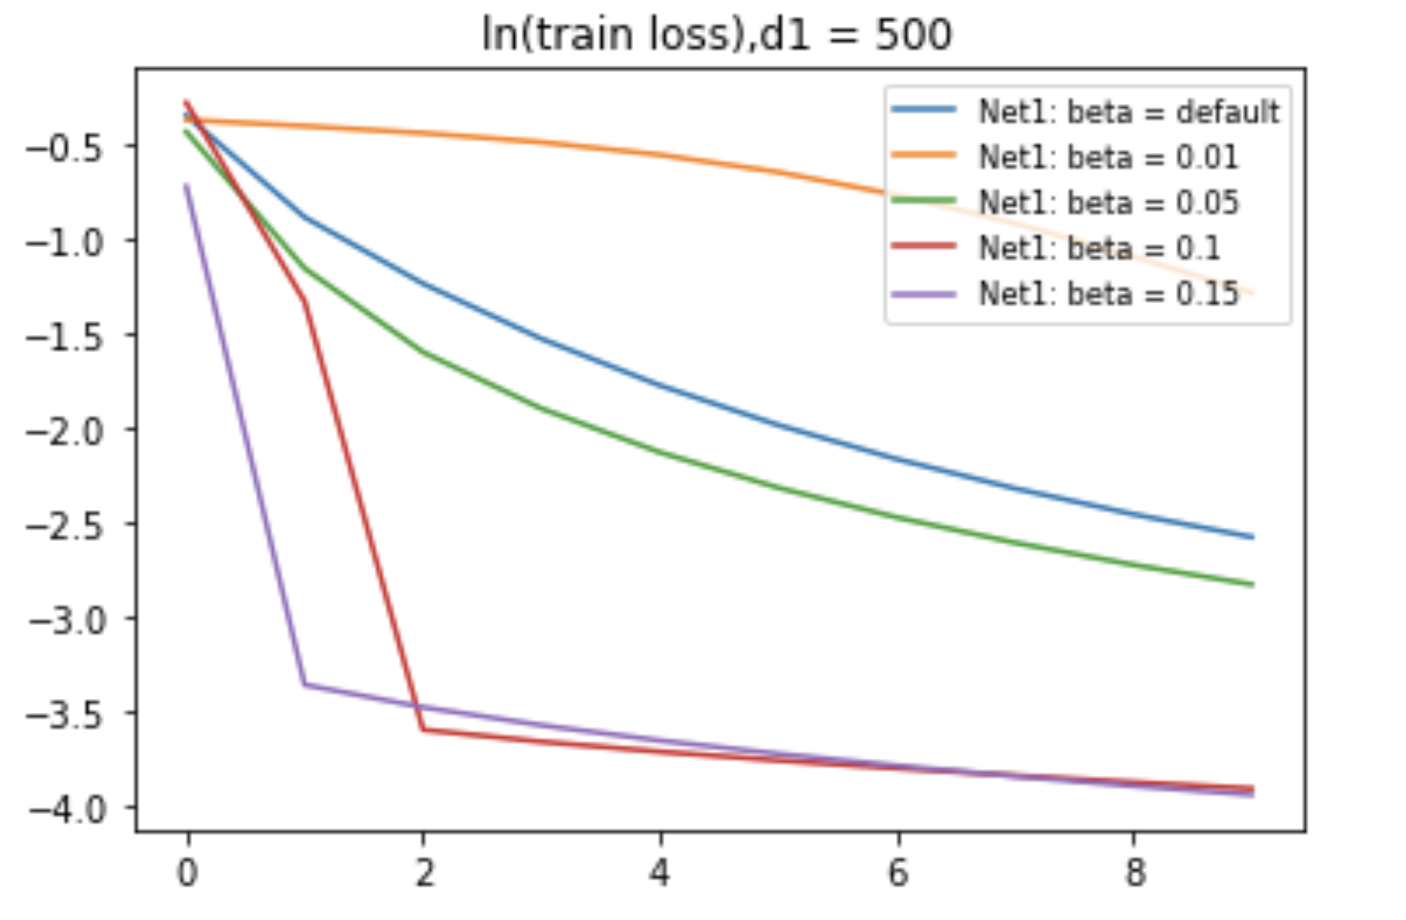
\includegraphics[width=1.5in]{MNIST_hidden500_uniform2.png}
	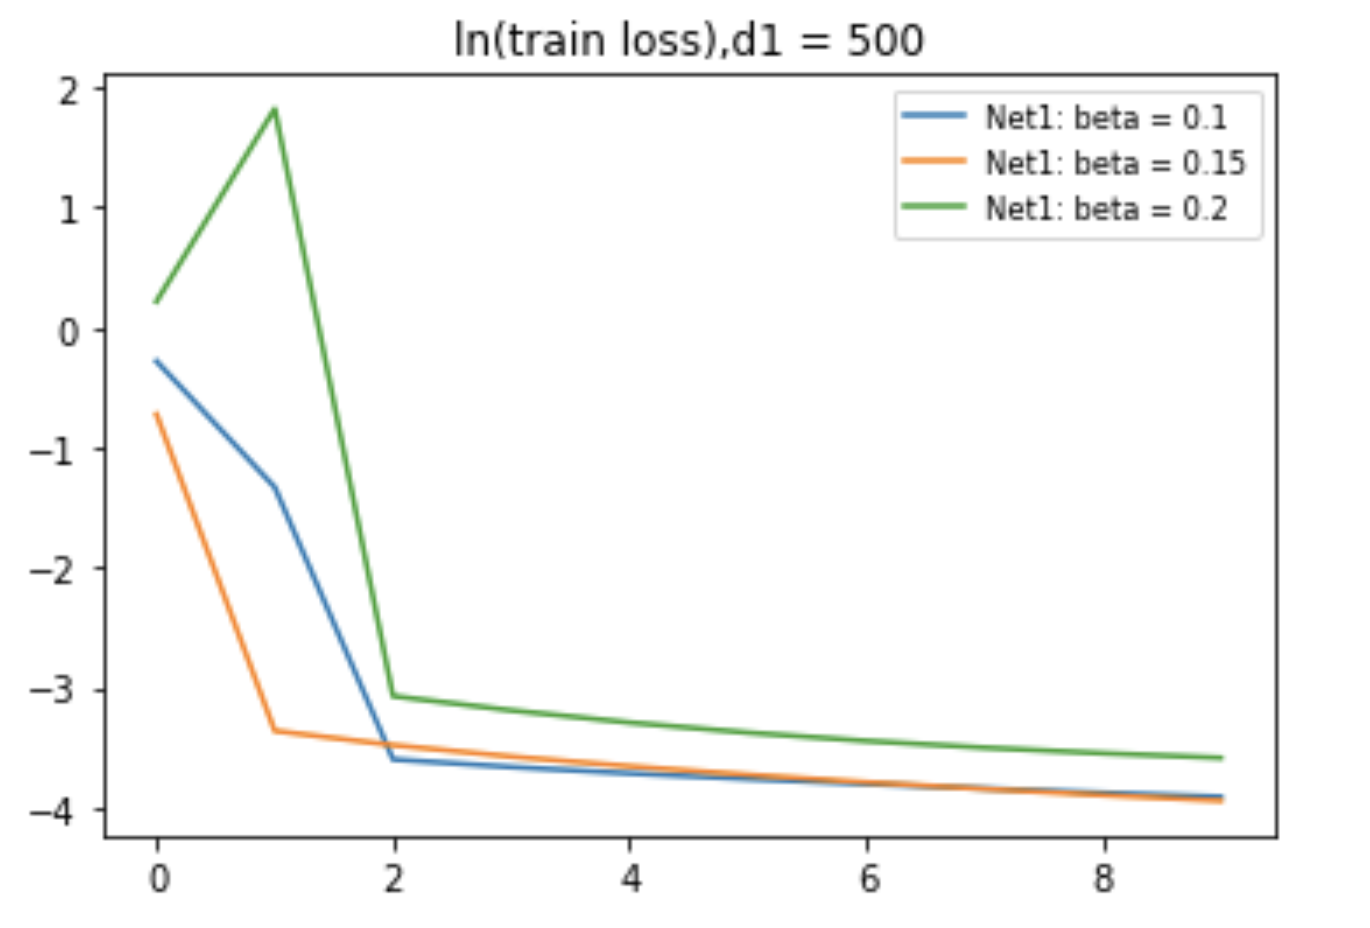
\includegraphics[width=1.5in]{MNIST_hidden500_uniform3.png}
	\caption{MNIST: $d_1 = 500$, $W_1,W_2,b \sim U(-\beta,\beta)$}
\end{figure}

 \begin{figure}[H]
	\centering
	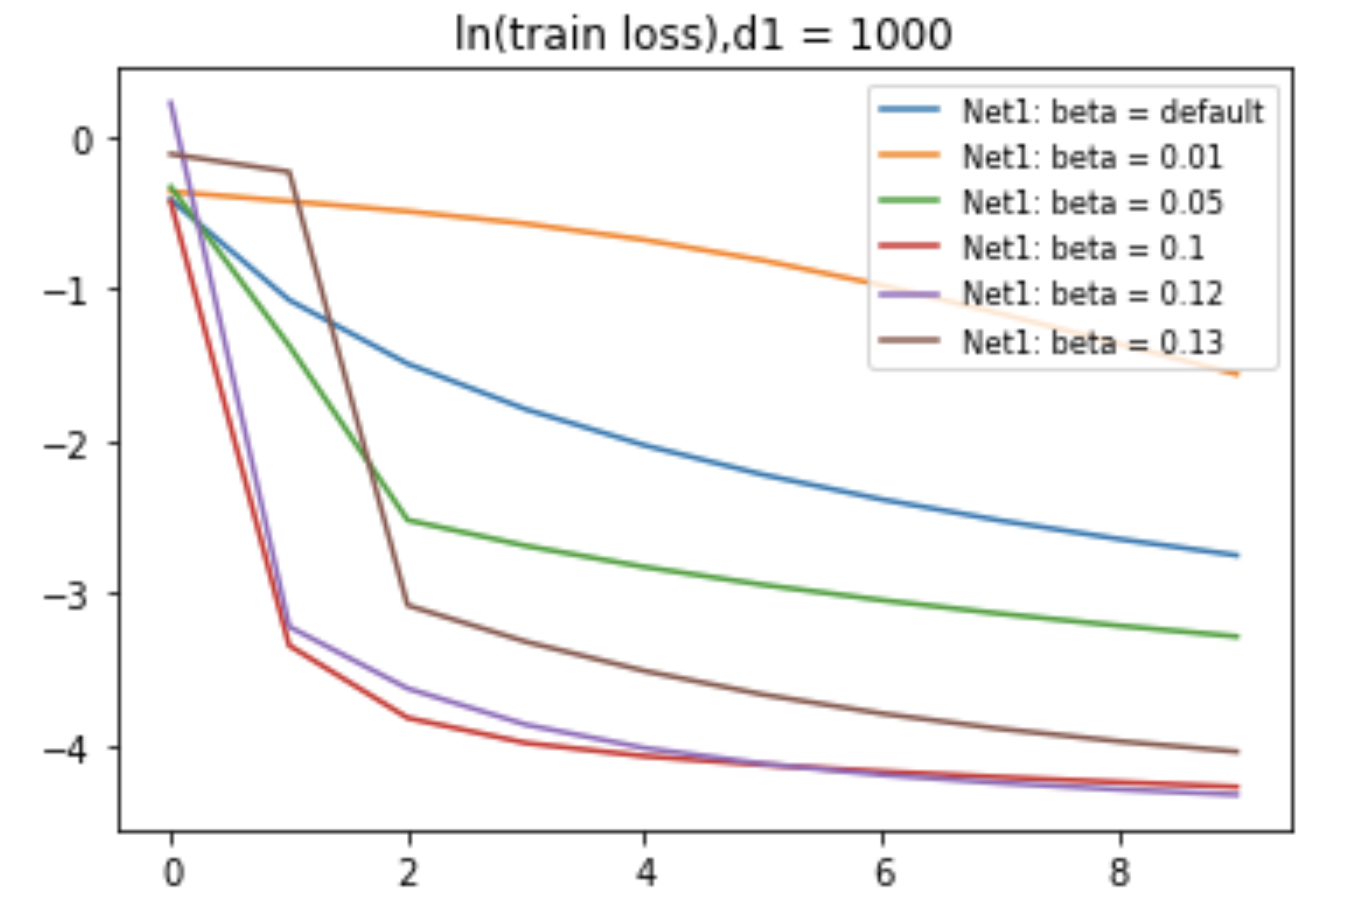
\includegraphics[width=1.5in]{MNIST_hidden1000_uniform1.png}
	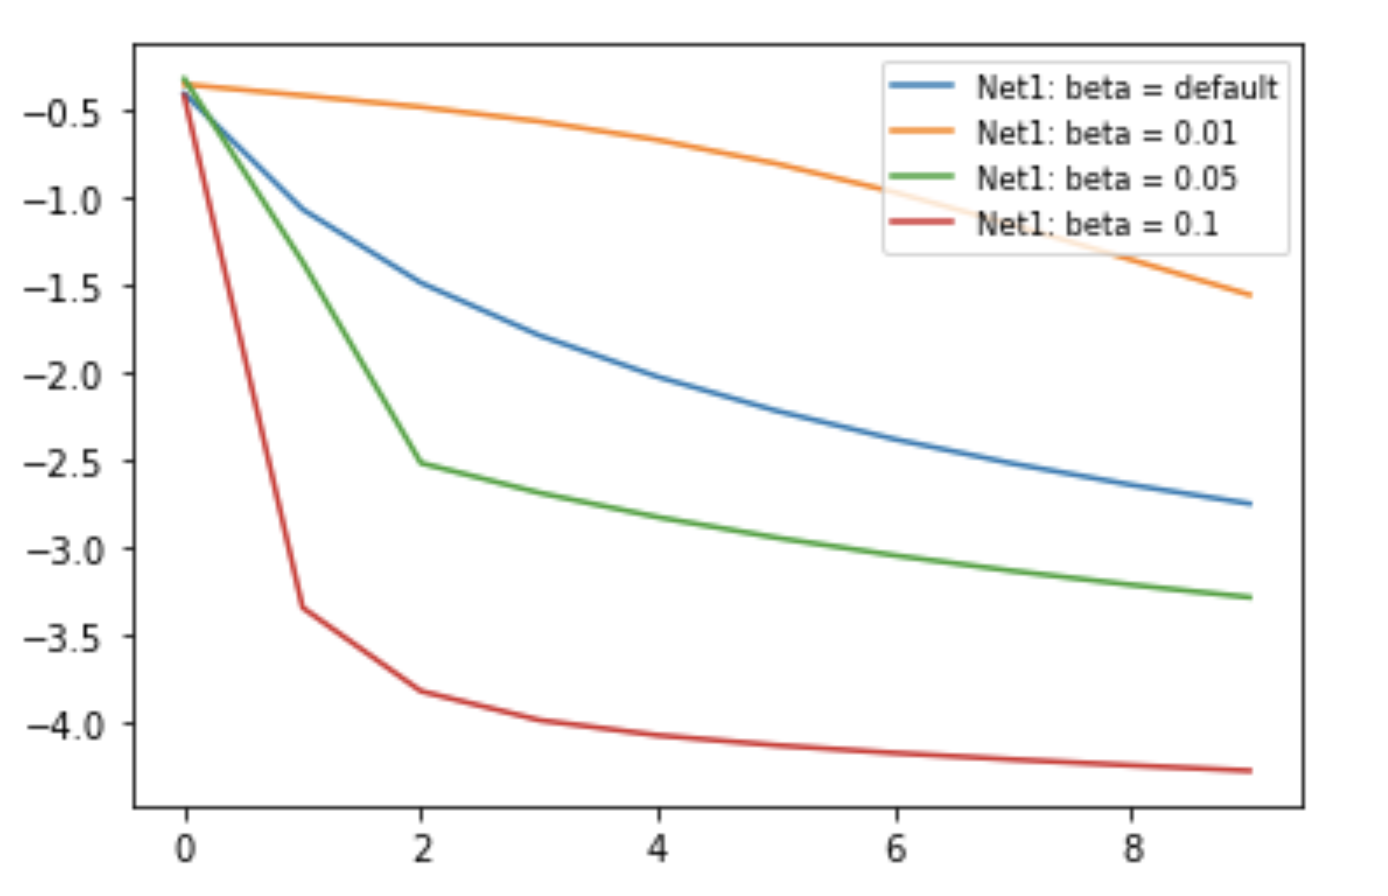
\includegraphics[width=1.5in]{MNIST_hidden1000_uniform2.png}
	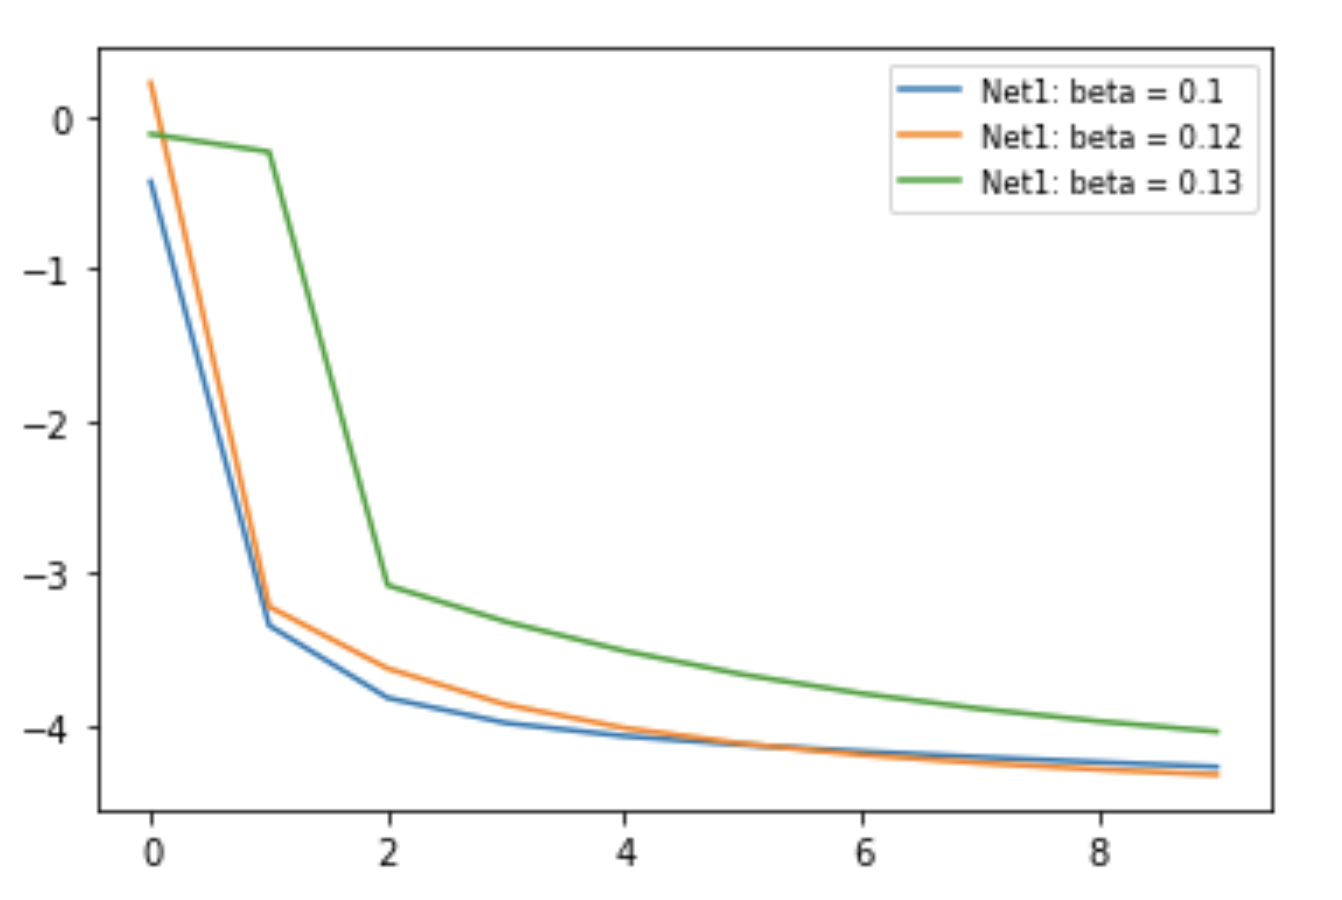
\includegraphics[width=1.5in]{MNIST_hidden1000_uniform3.png}
	\caption{MNIST: $d_1 = 1000$, $W_1,W_2,b \sim U(-\beta,\beta)$}
\end{figure}
 
  \begin{figure}[H]
 	\centering
 	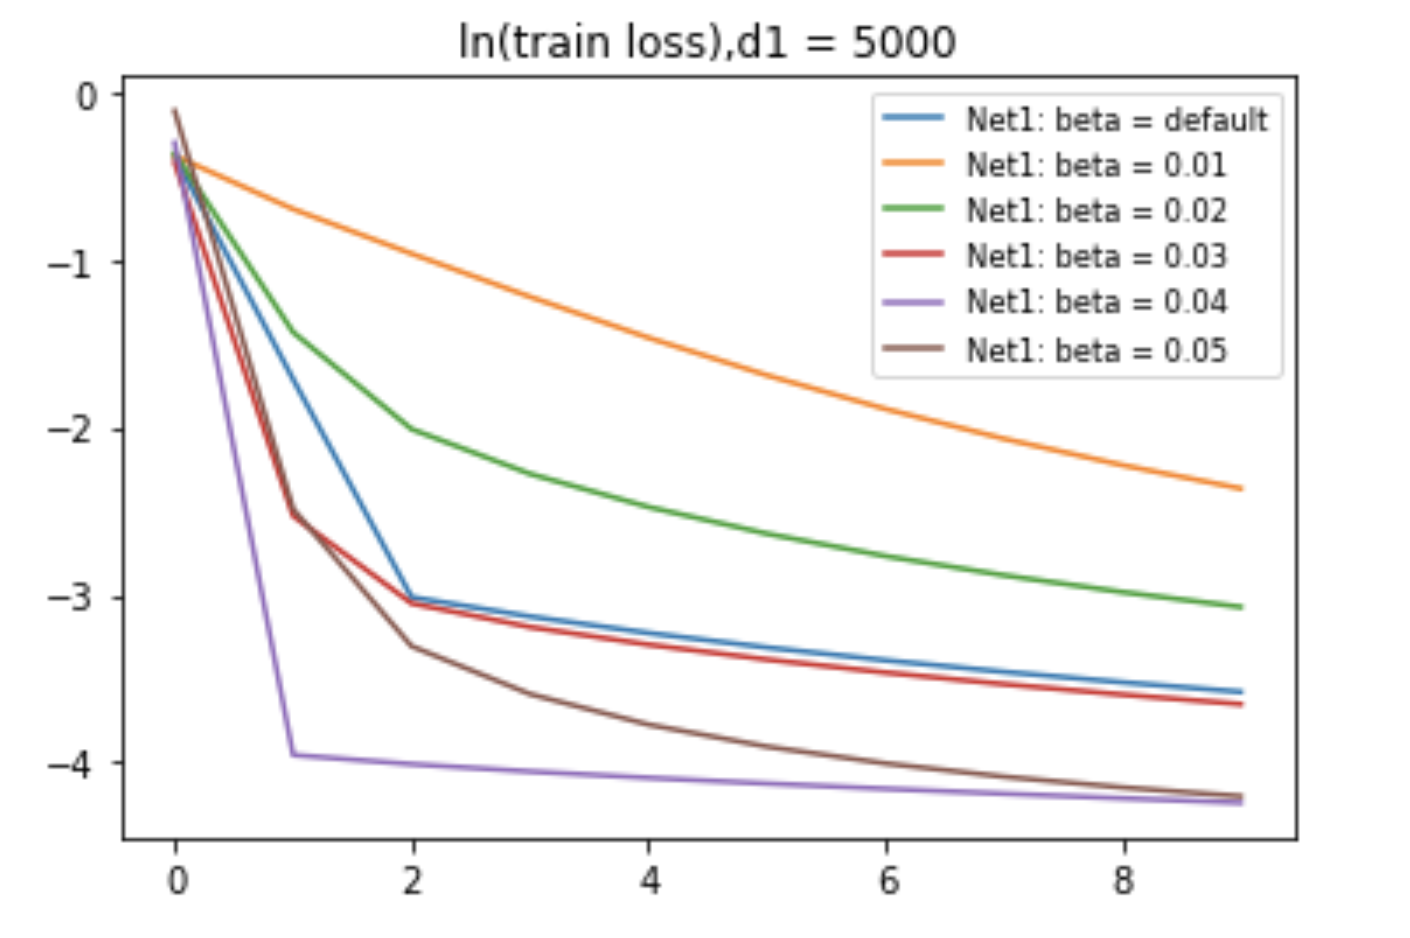
\includegraphics[width=1.5in]{MNIST_hidden5000_uniform1.png}
 	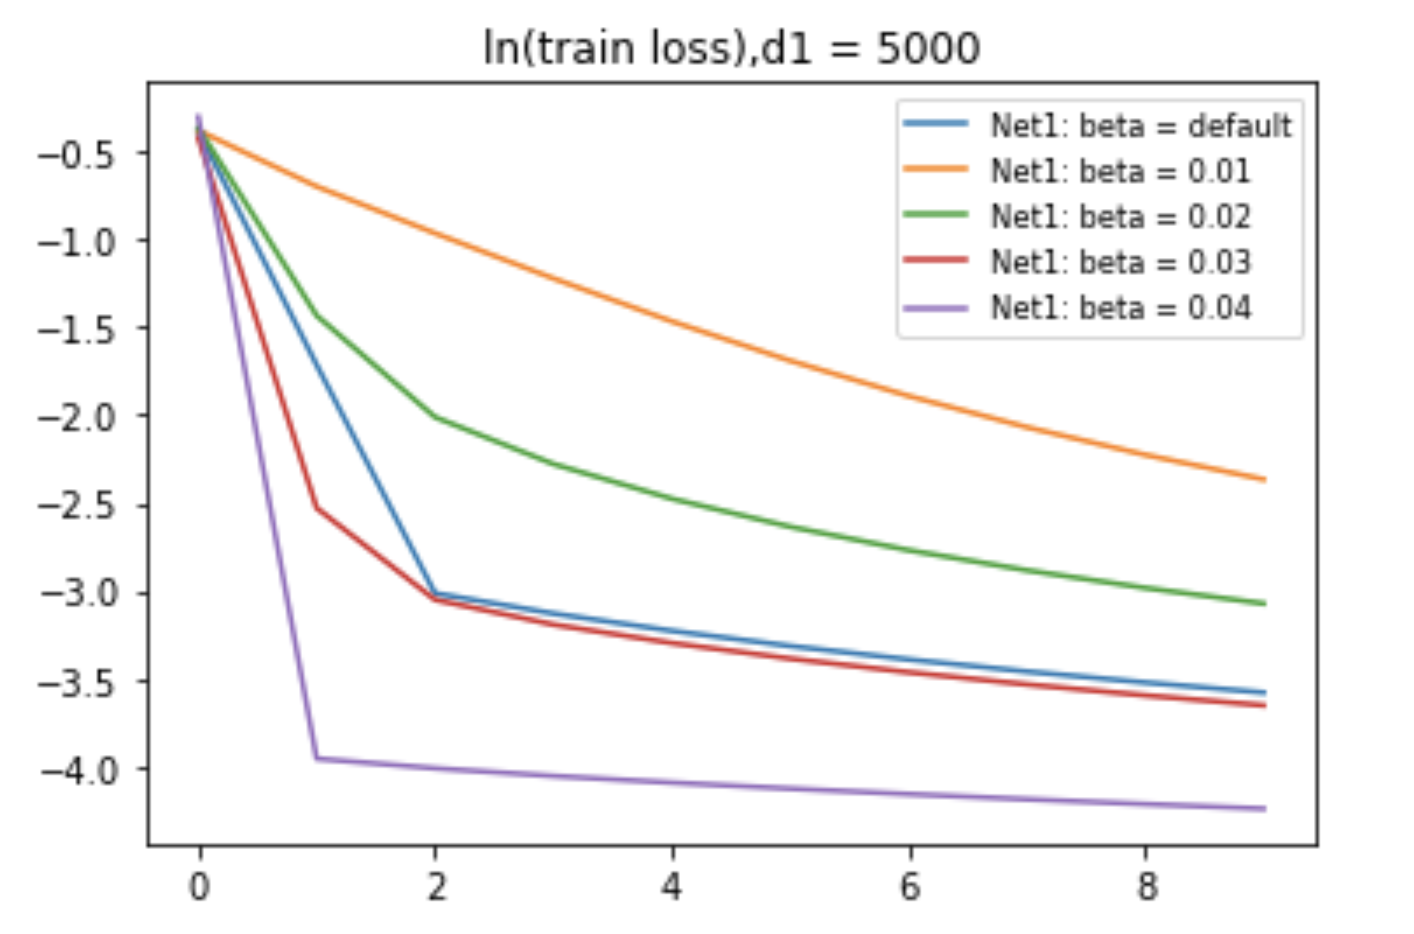
\includegraphics[width=1.5in]{MNIST_hidden5000_uniform2.png}
 	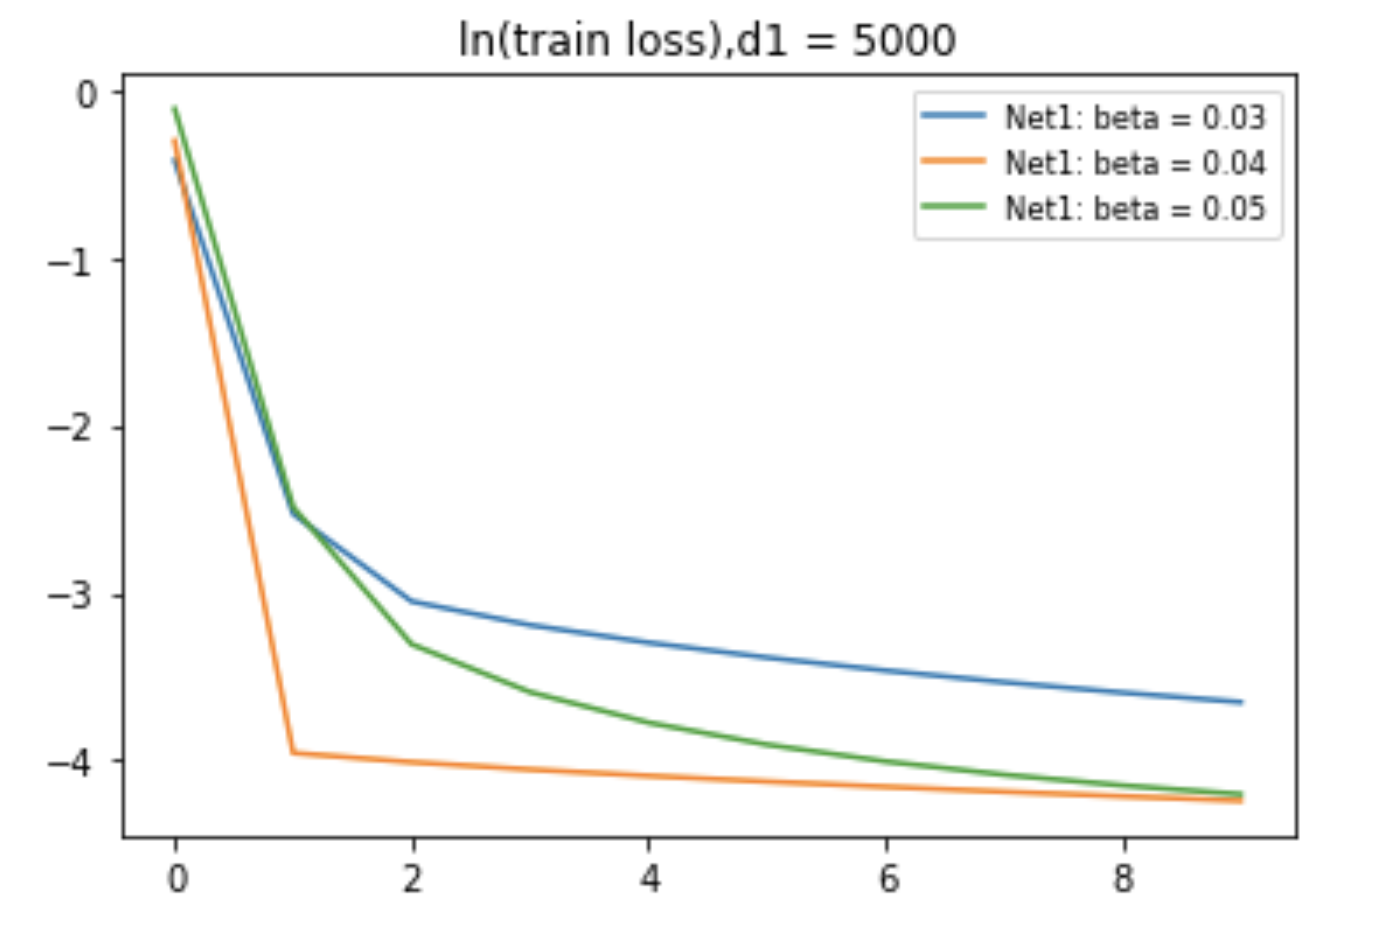
\includegraphics[width=1.5in]{MNIST_hidden5000_uniform3.png}
 	\caption{MNIST: $d_1 = 5000$, $W_1,W_2,b \sim U(-\beta,\beta)$}
 \end{figure}
 
   \begin{figure}[H]
 	\centering
 	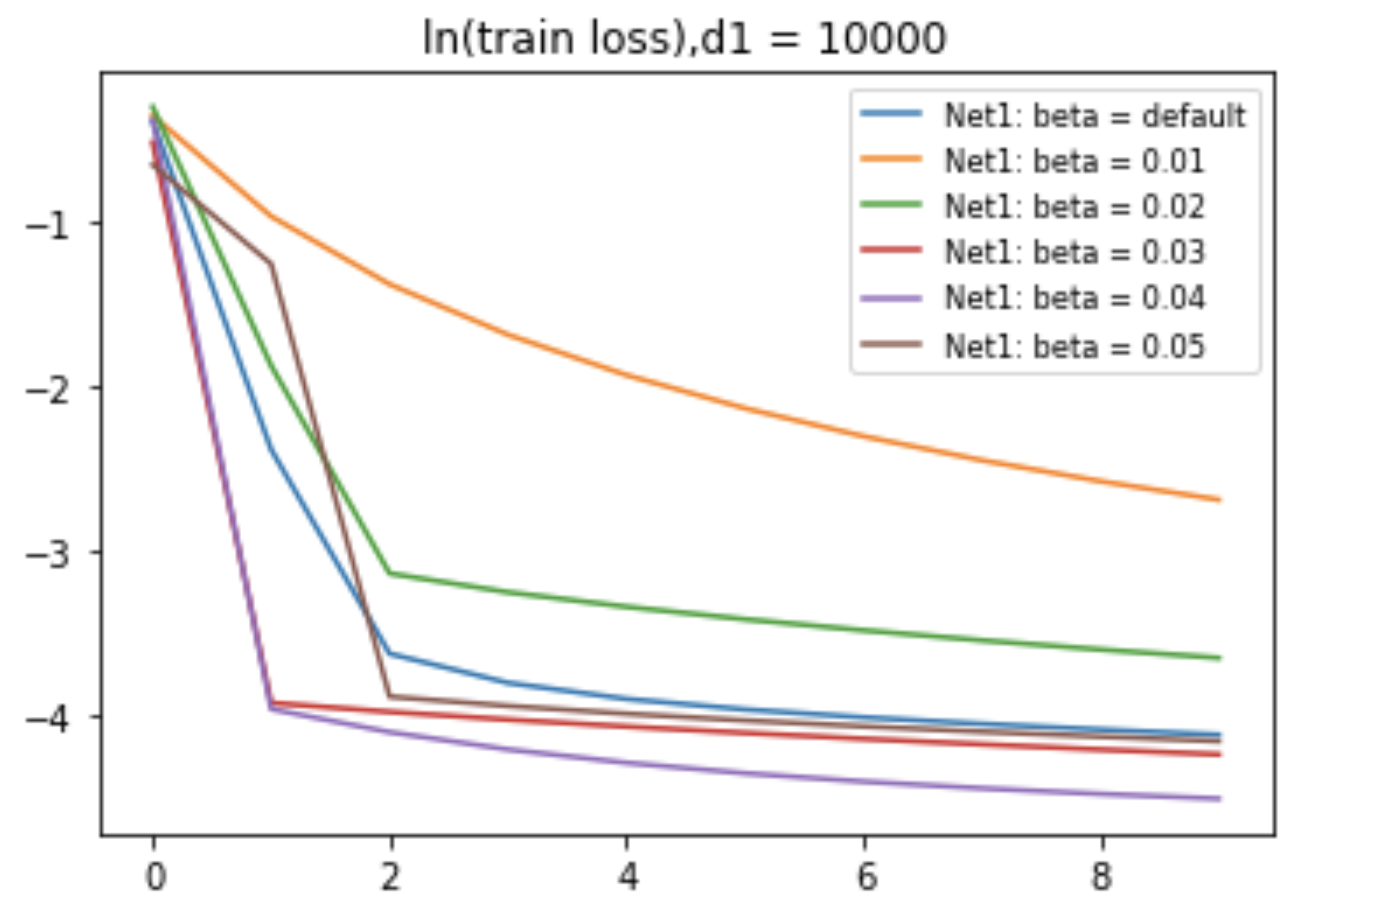
\includegraphics[width=1.5in]{MNIST_hidden10000_uniform1.png}
 	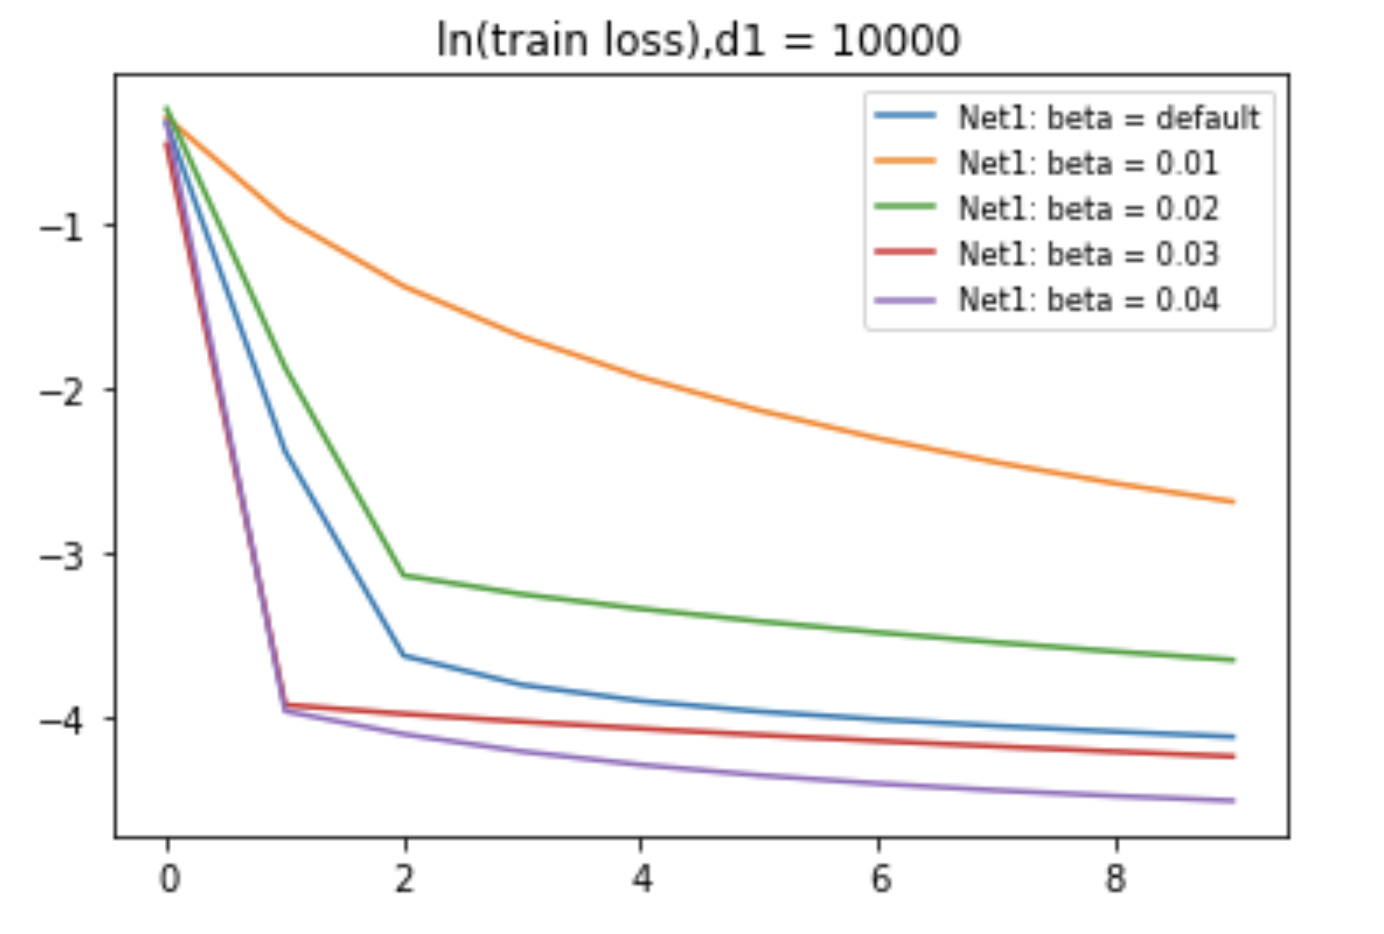
\includegraphics[width=1.5in]{MNIST_hidden10000_uniform2.png}
 	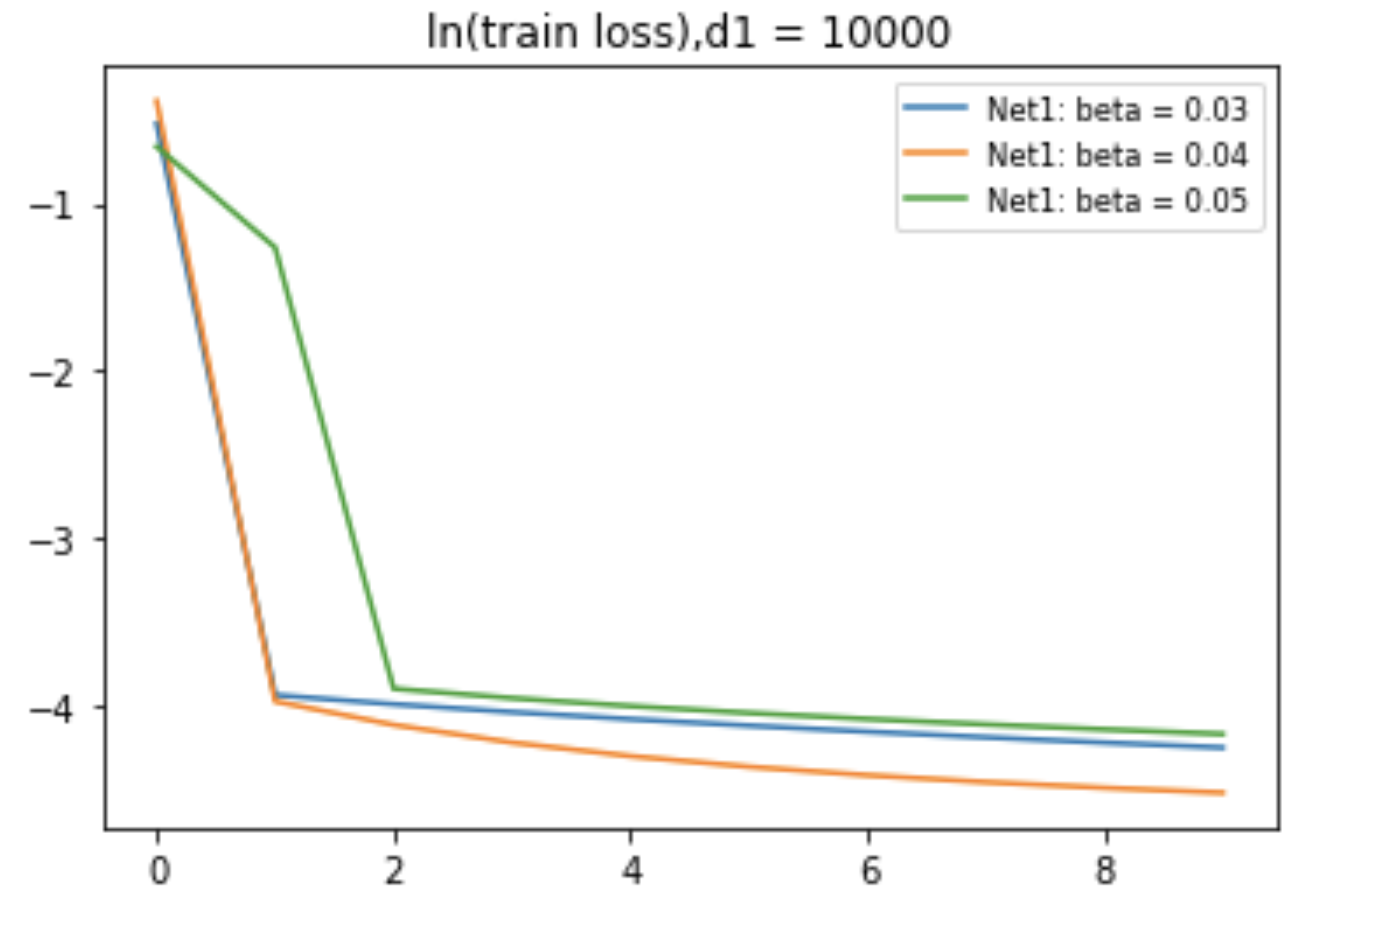
\includegraphics[width=1.5in]{MNIST_hidden10000_uniform3.png}
 	\caption{MNIST: $d_1 = 10000$, $W_1,W_2,b \sim U(-\beta,\beta)$}
 \end{figure}

   \begin{figure}[H]
	\centering
	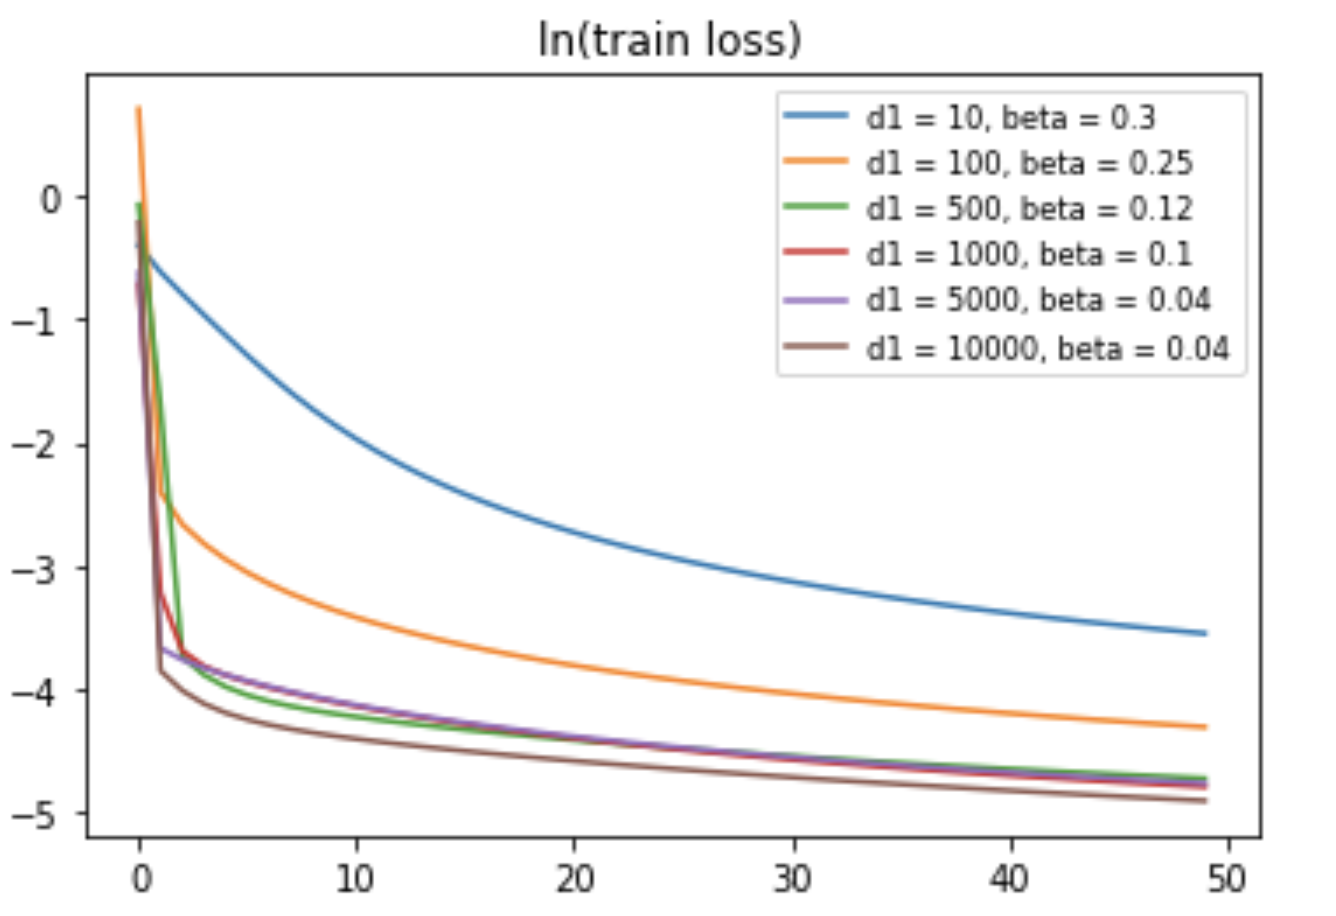
\includegraphics[width=1.5in]{MNIST_1hidden_step50_uniform1.png}
	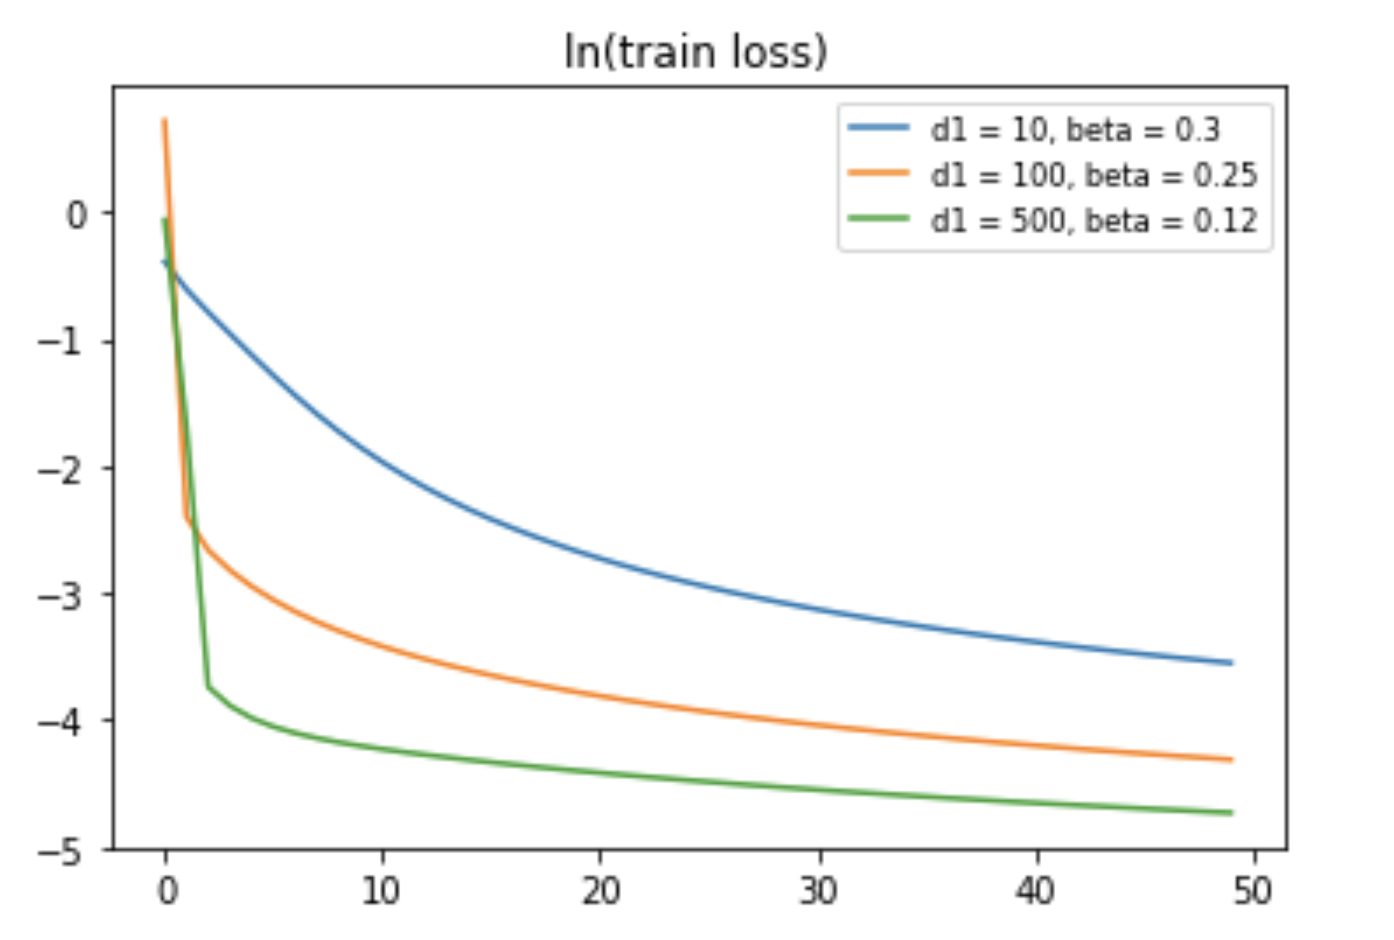
\includegraphics[width=1.5in]{MNIST_1hidden_step50_uniform2.png}
	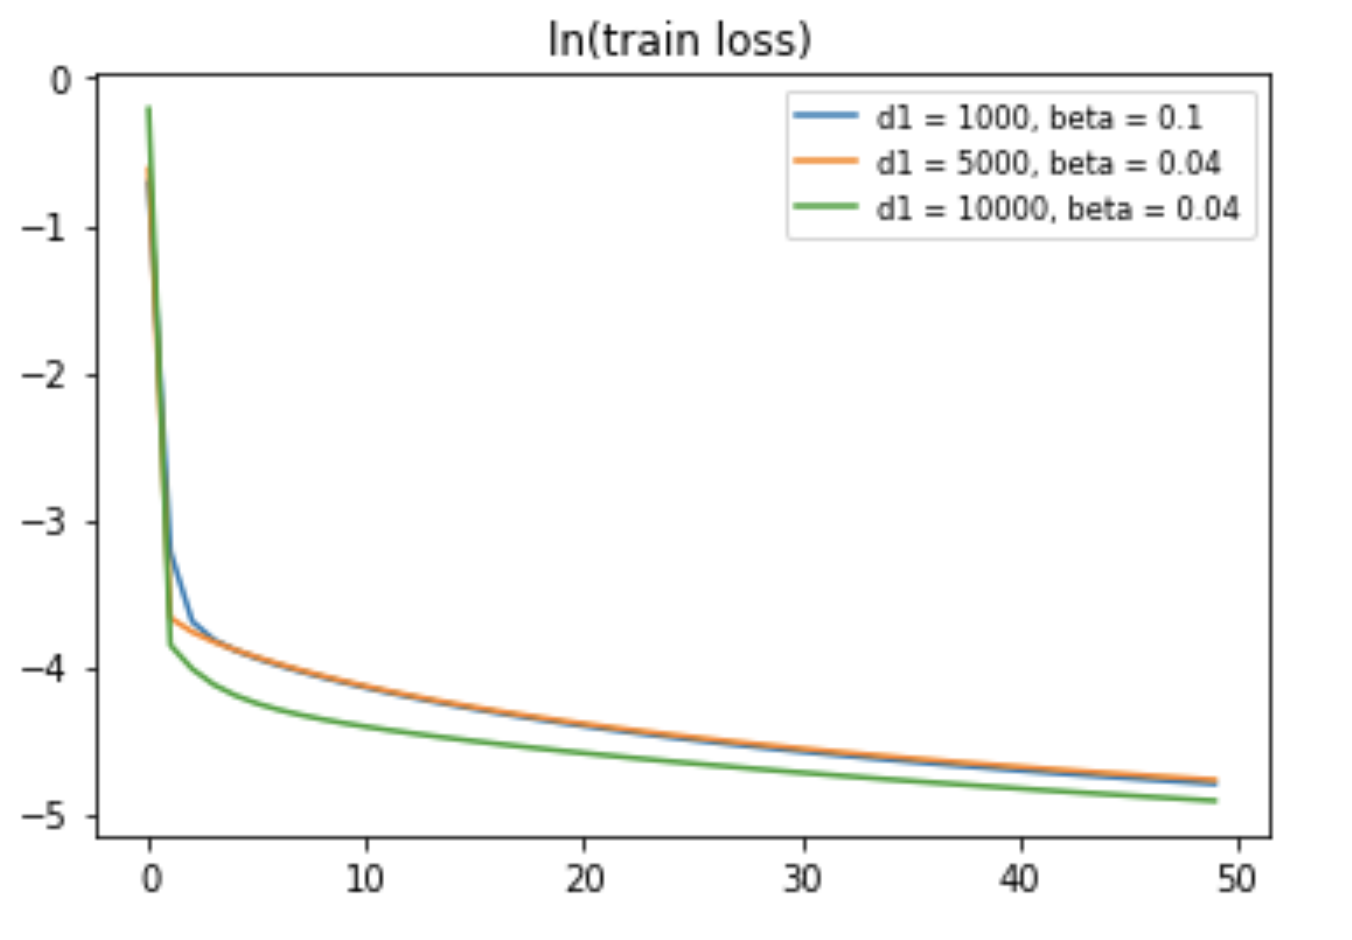
\includegraphics[width=1.5in]{MNIST_1hidden_step50_uniform3.png}
	\caption{MNIST: $d_1 = 10,100,500,1000,5000,10000$, $W_1,W_2,b \sim U(-\beta,\beta)$}
\end{figure}
 
    \begin{figure}[H]
 	\centering
 	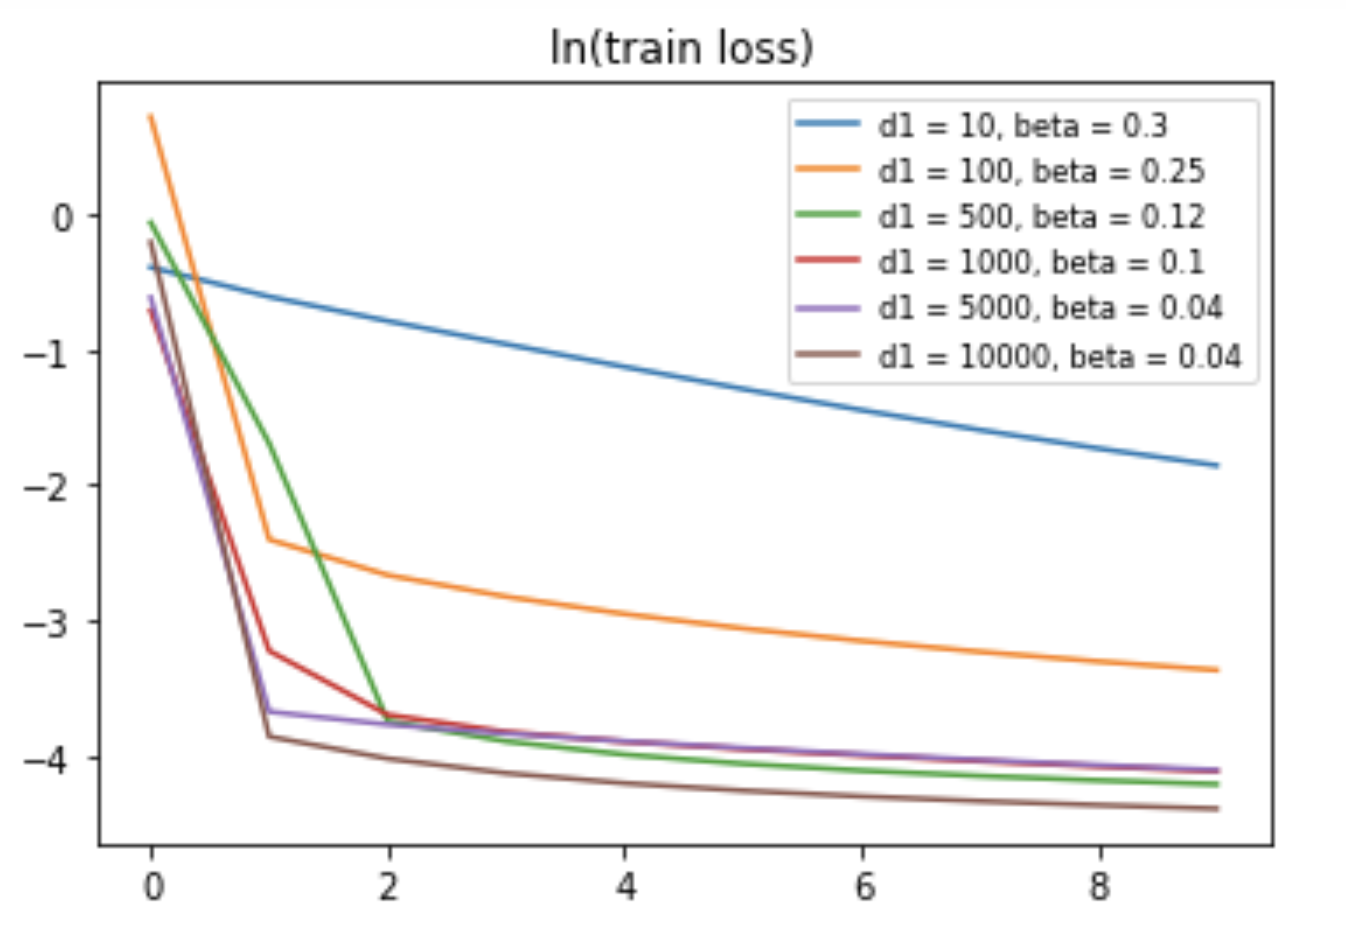
\includegraphics[width=1.5in]{MNIST_1hidden_step10_uniform1.png}
 	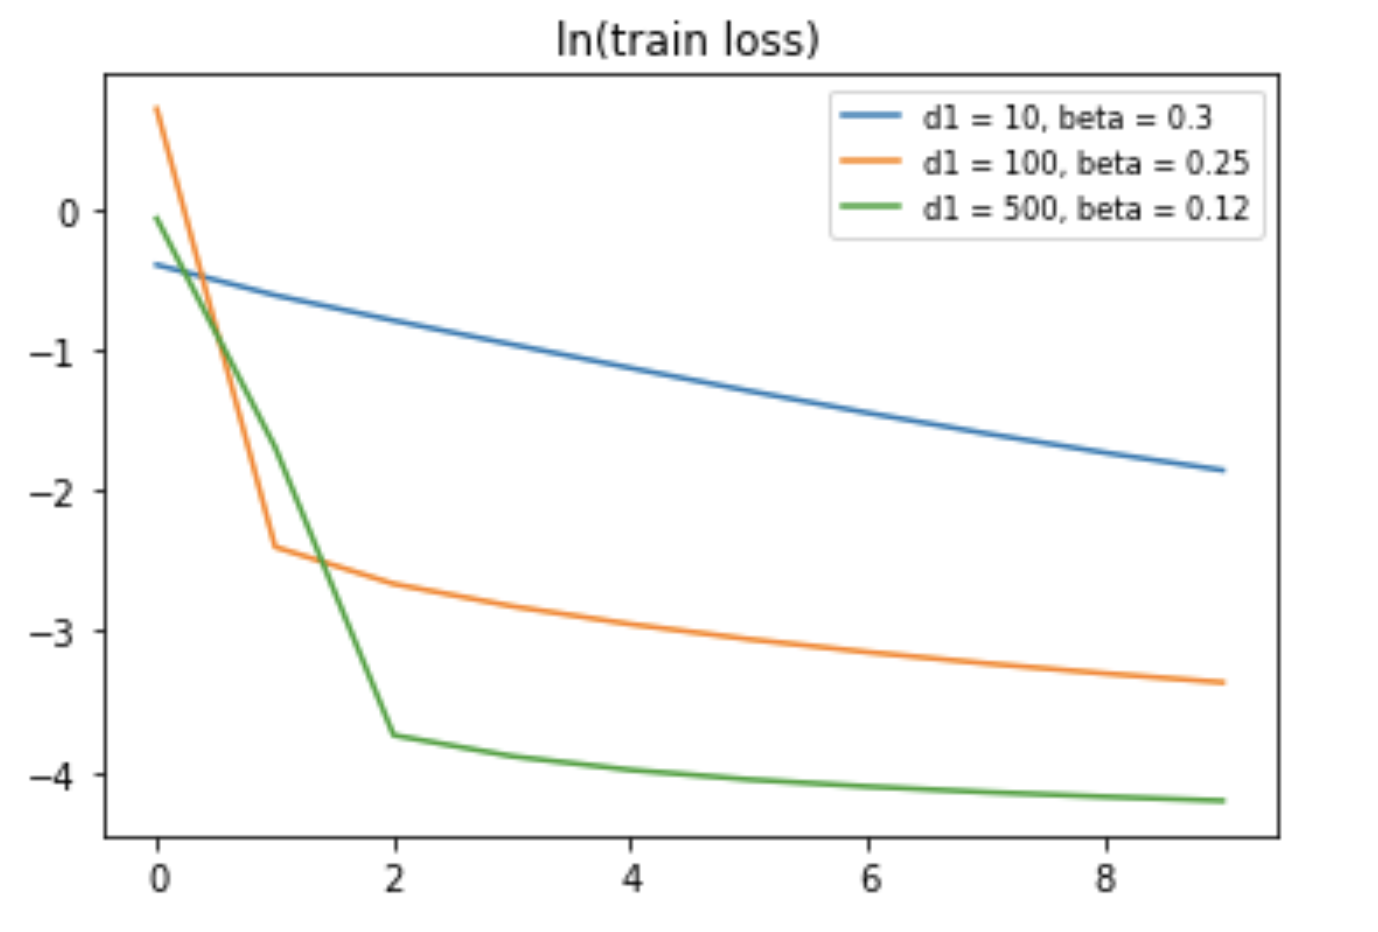
\includegraphics[width=1.5in]{MNIST_1hidden_step10_uniform2.png}
 	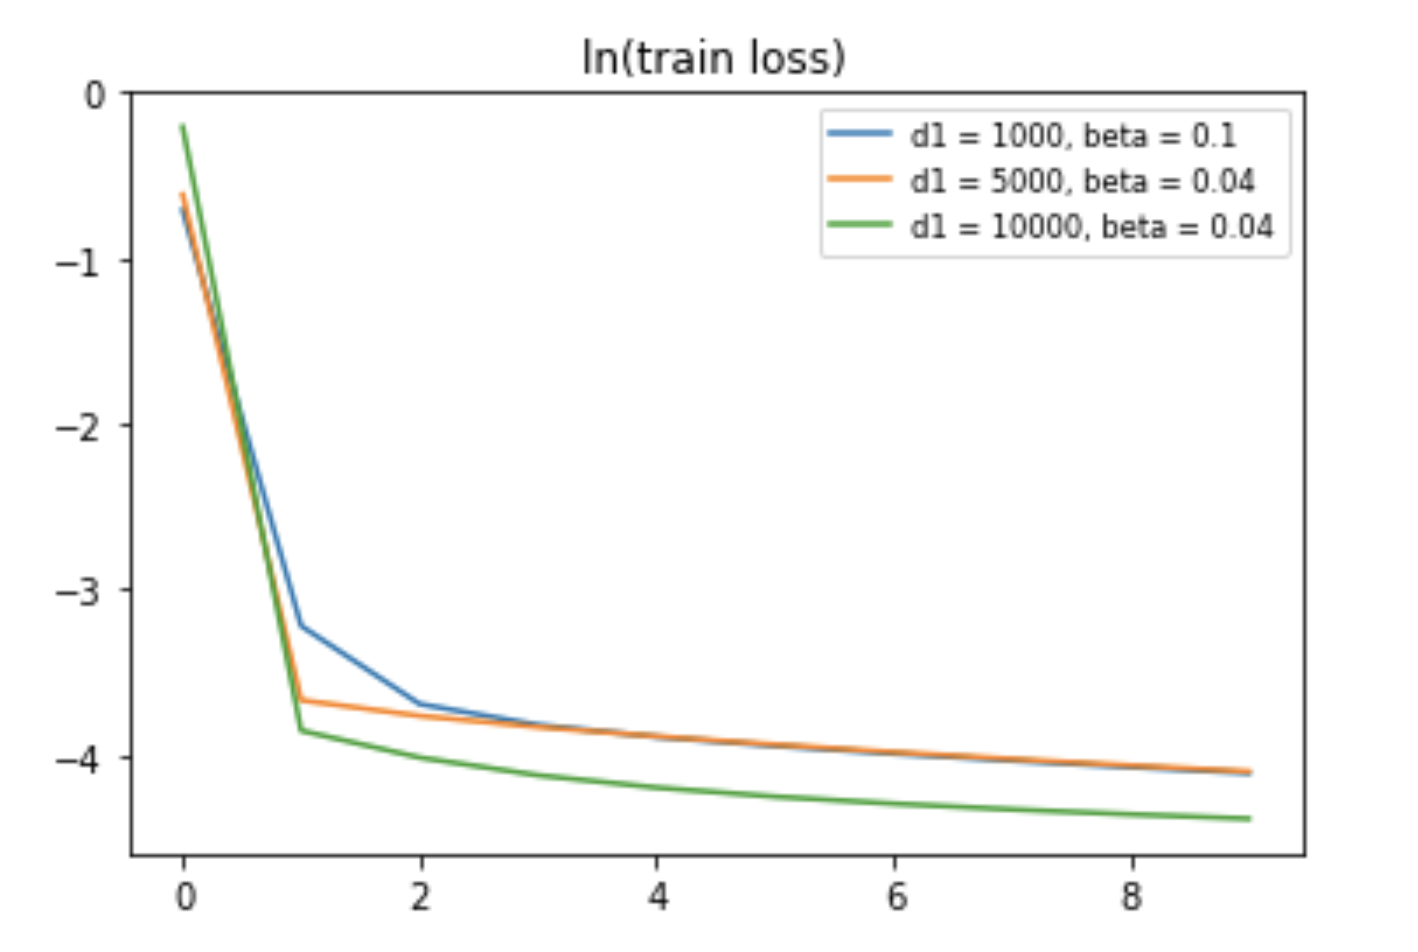
\includegraphics[width=1.5in]{MNIST_1hidden_step10_uniform3.png}
 	\caption{MNIST: $d_1 = 10,100,500,1000,5000,10000$, $W_1,W_2,b \sim U(-\beta,\beta)$}
 \end{figure}
 